\chapter{Design and Implementation}
\section{Timescale}
\label{section:timescale_system_architecture}

\subsection{Entity-Relationship (ER) diagram}
\begin{figure}[h]
    \centering
    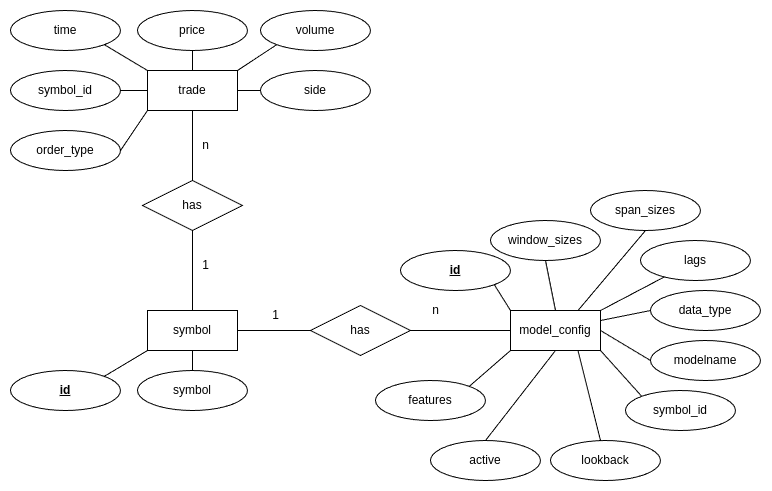
\includegraphics[width=\textwidth]{figures/ER-diagram.png}
    \caption{ER Diagram}
    \label{fig:er_diagram}
\end{figure}

The Entity-Relationship (ER) diagram establishes the database schema, which is designed for the storage and analysis of financial transactions. At its core is the \texttt{trade} entity essential for the transactional attributes: time, price, volume, linked via a \texttt{symbol\_id} to the corresponding currency pair in the \texttt{symbol} entity. This entity, with its unique identifier and descriptive nomenclature, categorizes the trades according to the traded financial instruments.

Accompanying the transactional data is the \texttt{model\_config} entity, which contains the configuration parameters critical for the predictive models utilized by the model service. Attributes defining the data's dimensions and historical scope, such as \texttt{span\_sizes}, \texttt{window\_sizes}, and \texttt{lags}, are specified to define the data features fed into the prediction models. The \texttt{model\_config's} direct association with the \texttt{symbol\_id} provides a unique configuration for each currency pair, facilitating the direct link between the predictive model and the financial instrument.

\subsection{Symbol Table}
The \texttt{symbol} table is defined as followed (Listing \ref{lst:symbol_table}), capturing the currency pairs.

\begin{lstlisting}[language=sql, caption=Symbol Table Structure, label=lst:symbol_table]
CREATE TABLE IF NOT EXISTS symbol (
    id SERIAL PRIMARY KEY,
    symbol TEXT NOT NULL UNIQUE
);

CREATE INDEX idx_symbol_symbol ON symbol (symbol);
\end{lstlisting}

This standard PostgreSQL table maintains a list of currency pairs like \texttt{ETH/USD}. An index is constructed to enhance the efficiency of queries, particularly when determining the associated \texttt{symbol\_id}.

\subsection{Model Configuration Table}
The structure of the \texttt{model\_config} table is delineated below (Listing \ref{lst:model_config_table}), encompassing the predictive model configurations:

\begin{lstlisting}[language=sql, caption=Model Configuration Table Structure, label=lst:model_config_table]
CREATE TABLE model_config (
    id SERIAL PRIMARY KEY,
    symbol_id SERIAL REFERENCES symbol(id),
    modelname TEXT,
    data_type TEXT,
    lookback INTEGER,
    lags INTEGER[],
    window_sizes INTEGER[],
    span_sizes INTEGER[],
    active BOOLEAN,
    features TEXT[]
);

ALTER TABLE model_config ADD CONSTRAINT model_config_constraint
UNIQUE (symbol_id, active);
\end{lstlisting}

This table not only records the configurations but also establishes a foreign key to the \texttt{symbol} table. A significant addition to the table is the unique constraint \texttt{model\_config\_constraint}, ensuring that only one configuration per \texttt{symbol\_id} can be marked as active at any given time. This enforces the exclusivity of active configurations, preventing conflicts and ambiguity in the model service operation. \\

The structure of the \texttt{trade} table  will be discussed in Section \ref{section:trade_table}, which focuses on hypertables. \\

In summary, the presented schema combines the transactional data with the intricacies of analytical model configurations, constructing a sophisticated data infrastructure for comprehensive financial analysis within the database.

\subsection{Hypertables}
Timescale introduces the concept of hypertables, a sophisticated abstraction over regular PostgreSQL tables specifically designed to enhance the management of time-series data. 

\begin{itemize}
    \item \textbf{Seamless Integration:} Hypertables blend in seamlessly with standard PostgreSQL tables, offering a dual-structure setup where each serves its distinct purpose. Users interact with hypertables just like regular tables, ensuring a familiar interface. This setup allows for efficient management of time-based data while maintaining the integrity and functionality of standard relational data storage.
    \item \textbf{Performance Optimization:} One of the primary advantages of hypertables is their ability to significantly improve insert and query performance. This is achieved through partitioning the time-series data based on the time dimension. Timescale efficiently manages the partitioning process behind the scenes, thereby abstracting the complexities involved in maintaining the hypertable's partitions.
\end{itemize}

In summary, hypertables in Timescale represent a pivotal innovation in the realm of time-series data management. They blend the familiarity of PostgreSQL tables with advanced time-based partitioning features, resulting in a powerful tool for efficient and effective time-series data handling.

\subsubsection{Trade Table:}
\label{section:trade_table}
\begin{lstlisting}[language=sql, caption=Trade Hypertable, label={lst:trade_hypertable}]
CREATE TABLE IF NOT EXISTS trade (
    time TIMESTAMPTZ NOT NULL,
    price DOUBLE PRECISION NOT NULL,  
    volume DOUBLE PRECISION NOT NULL, 
    side VARCHAR(1),
    order_type VARCHAR(1),
    symbol_id SERIAL NOT NULL
);

CREATE INDEX idx_trade_symbol_id ON trade (time, symbol_id);

SELECT create_hypertable('trade', 'time', migrate_data => true);
\end{lstlisting}

\begin{itemize}
\item \textbf{time}: The timestamp of the trade, essential for time-series analysis.
\item \textbf{price}: The price at which the trade occurred.
\item \textbf{volume}: The volume of the trade.
\item \textbf{side}: A variable indicating the trade side (e.g. buy or sell).
\item \textbf{order\_type}: The type of order executed in the trade (e.g. limit or market order).
\item \textbf{symbol\_id}: A unique identifier for the traded symbol.
\end{itemize}

In the early stages of this project the price and volume were stored using the PostgreSQL Numeric type. This choice was initially made due to the high precision of the Numeric type, which is particularly suitable for financial data where accuracy is paramount. However, it was observed that while the Numeric type ensures precision, it is not the optimal choice to use in Timescale, especially in the context of time-series data \cite{timescale_best_practices}. \newline

The primary challenge with the Numeric type in Timescale arises from its impact on performance. The performance impact is particularly noticeable when executing continuous aggregates on larger datasets. Continuous aggregates are fundamental in time-series databases for efficient data analysis, but the use of the Numeric type significantly hampers the performance of these operations. The larger storage size and processing requirements of the Numeric type, as compared to \texttt{DOUBLE PRECISION}, contribute to this performance degradation. \newline

As a result of these insights, the data type for price and volume was transitioned to \texttt{DOUBLE PRECISION}. This change strikes a balance between the need for precision and performance, which is crucial for time-series analysis in Timescale. \newline

Furthermore, the choice of \texttt{TIMESTAMPTZ} for time-stamping the data aligns with the best practices recommended for Timescale hypertables. The \texttt{TIMESTAMPTZ} data type, which stores both timestamp and timezone information, is particularly well suited for time-series data as it ensures accurate representation and manipulation of time, considering the time zone differences. This is essential in financial applications where transactions may span multiple time zones and accurate time-stamping is critical for analysis and reporting. \newline

Another optimization was storing only the \texttt{symbol\_id} instead of the full symbol (e.g., \texttt{ETH/USD}) in the database, as it significantly reduces data redundancy and optimizes query performance by referencing a compact, unique identifier for each trading pair.  

% see source https://www.timescale.com/blog/best-practices-for-picking-postgresql-data-types/  

\paragraph{Rationale for using a Hypertable:}
\begin{itemize}
\item \textbf{Time-based Partitioning}: As trades are inherently time-stamped the hypertable efficiently partitions data based on time, facilitating faster query performance, especially for time-bound data retrievals.
\item \textbf{Scalability}: With continuous growth in the trade data table, hypertables offer scalable solutions to manage large volumes of data without compromising on performance.
\item \textbf{Optimized Queries}: The creation of an index on the time and symbol\_id columns significantly enhances the query performance, especially for operations like range queries, which are common in financial analyses.
\item \textbf{Aggregation Support}: Hypertables are adept at handling aggregations, which are crucial for calculating OHLC (open, high, low, close) metrics, volume, and trade counts from raw trade data.
\end{itemize}

In essence, the utilization of a hypertable for the trade table in Timescale aligns with the requirements of time-series data handling in financial contexts. It provides an efficient, scalable, and performance-optimized framework for storing and querying trade data, thereby supporting intricate financial analysis and reporting.

\subsection{Materialized Views and Continuous Aggregates}

In the realm of time-series data management, especially in financial databases where data is voluminous and frequently accessed, optimizing query performance is crucial. Materialized Views and Continuous Aggregates in Timescale offer a potent solution for this challenge. These tools enable efficient data aggregation and faster retrieval by storing query results and refreshing them at regular intervals. This approach is particularly beneficial in scenarios involving repetitive and computationally intensive queries, such as aggregating trade data into OHLC (Open, High, Low, Close) metrics.

\subsubsection{OHLC Hourly Aggregation}
\label{section:ohlc_hourly_agg}
A materialized view named \texttt{ohlc\_hour} (Listing \ref{lst:ohlc_hour_materialized_view}) is utilized to aggregate trade data into hourly OHLC metrics. The view is created with the following characteristics:

\begin{lstlisting}[language=sql, caption=OHLC Materialized View, label={lst:ohlc_hour_materialized_view}]
CREATE MATERIALIZED VIEW ohlc_hour
WITH (timescaledb.continuous, timescaledb.create_group_indexes=TRUE, timescaledb.finalized=TRUE) AS
    SELECT
        time_bucket('1 hour', time) AS bucket,
        symbol_id,
        FIRST(price, time) AS open_price,
        MAX(price) AS high, 
        MIN(price) AS low,
        LAST(price, time) AS close_price,
        SUM(volume) AS volume,
        CAST(COUNT(*) AS INTEGER) AS count 
    FROM trade
GROUP BY bucket, symbol_id; 
\end{lstlisting}
\mbox{} \\
Key aspects of this view include:
\begin{itemize}
\item \textbf{Time Bucketing}: Aggregating trades into one-hour intervals.
\item \textbf{Data Accuracy}: The \texttt{finalized=TRUE} setting ensures that only fully aggregated data (complete hours) are returned.
\item \textbf{Trade Metrics}: Calculating open-, high-, low-, close-price, total volume, and trade count for each symbol within each time bucket.
\item \textbf{Overflow Consideration}: The trade count is cast to an integer, which has the potential for an overflow if the trade volume is exceedingly high, but after the analysis of the \texttt{ETH/USD} trades from the last couple of years the highest trade count in one hour was 25.000 trades which is nowhere close to the largest integer value of 2147483647.
\end{itemize}

Overall this materialized view reduces the raw trade data into a more manageable presentation, which will be utilized as a dataset for training the prediction models. 

\subsubsection{Continuous Aggregate Policy}
To maintain and update the \texttt{ohlc\_hour} view, a continuous aggregate policy is implemented (Listing \ref{lst:ohlc_hour_continuous_aggregate_policy}).

\begin{lstlisting}[language=sql, caption=OHLC Continuous Aggregate Policy, label={lst:ohlc_hour_continuous_aggregate_policy}]
SELECT add_continuous_aggregate_policy('ohlc_hour',
    start_offset => INTERVAL '3 hour', 
    end_offset => INTERVAL '1 hour',
    schedule_interval => INTERVAL '1 hour');
\end{lstlisting}
\mbox{} \\
This policy dictates:
\begin{itemize}
\item \textbf{Data Freshness}: Data is aggregated and refreshed every hour.
\item \textbf{Time Offsets}: Determines the range of data being aggregated, ensuring timely updates without processing very recent data that may still be incomplete.
\end{itemize}

Through the implementation of Materialized Views and Continuous Aggregates, the database efficiently processes and provides quick access to vital financial metrics, enhancing the system's performance and responsiveness for time-series analysis.

\subsection{Procedures and Functions}
\subsubsection{Symbol}
Efficient symbol management within the database is facilitated through the implementation of specialized functions, particularly the \texttt{insert\_symbol} function (Listing \ref{lst:insert_symbol_function}). This function is pivotal for insertion of new symbols into the \texttt{symbol} table and retrieving their identifiers.

\begin{lstlisting}[language=SQL, caption={Function for Inserting New Symbols}, label={lst:insert_symbol_function}]
CREATE OR REPLACE FUNCTION insert_symbol(input_symbol TEXT)
RETURNS TABLE(out_id INTEGER, out_symbol TEXT)
LANGUAGE plpgsql AS $$
BEGIN
    -- Attempt to insert the new symbol
    INSERT INTO symbol (symbol)
    VALUES (input_symbol)
    ON CONFLICT (symbol) DO NOTHING
    RETURNING id INTO out_id;
    -- If insertion did not occur due to a conflict, select the existing symbol
    IF NOT FOUND THEN
        RETURN QUERY SELECT id, symbol FROM symbol WHERE symbol = input_symbol;
    ELSE
        -- Set output symbol as the input symbol and return the record
        out_symbol := input_symbol;
        RETURN NEXT;
    END IF;
END;
$$;
\end{lstlisting}
\mbox{} \\
The function operates under two scenarios:
\begin{itemize}
    \item On receiving a new symbol, it attempts an insertion. If successful, the function returns the identifier of the newly inserted symbol.
    \item If the symbol pre-exists, indicated by a conflict, the function refrains from insertion and instead queries the identifier of the existing symbol.
\end{itemize}

Utilizing the \texttt{ON CONFLICT} clause ensures that the database maintains unique symbols, thus preserving data integrity. This function exemplifies the database's capability to manage symbols efficiently by preventing duplicate entries and streamlining the insertion process.


\subsubsection{Insert Trade Procedure}
To facilitate the addition of new trade data into the database, the \texttt{insert\_trade} procedure (Listing \ref{lst:insert_trade_procedure}) is implemented, which  is crucial for the collector service to insert trade transactions efficiently. 
\begin{lstlisting}[language=SQL, caption={Procedure for Inserting Trade Data}, label=lst:insert_trade_procedure]
CREATE OR REPLACE PROCEDURE insert_trade (
    _time TIMESTAMPTZ,
    _price DOUBLE PRECISION,  
    _volume DOUBLE PRECISION, 
    _side VARCHAR(1),
    _order_type VARCHAR(1),
    _symbol_id INTEGER 
)
LANGUAGE plpgsql AS $$
BEGIN
    INSERT INTO trade (time, price, volume, side, order_type, symbol_id) 
    VALUES (_time, _price, _volume, _side, _order_type, _symbol_id);
END;
$$;
\end{lstlisting}

This procedure requires trade-related parameters such as the timestamp, price, volume, trade side, order type, and the associated symbol identifier. Upon invocation, it performs a straightforward insertion of the provided data into the \texttt{trade} table. \\

Key Features:
\begin{itemize}
    \item \textbf{Efficiency in Data Entry}: By encapsulating the insertion logic within a procedure, the process of adding new trades to the database is streamlined, ensuring rapid and error-free data entry.
    \item \textbf{Parameterized Inputs}: The procedure utilizes parameterized inputs, which not only enhance the clarity of the data being inserted but also aid in maintaining consistency and data integrity.
\end{itemize}

The \texttt{insert\_trade} procedure plays an integral role in managing the influx of trade data, ensuring that the database is continuously updated with the latest transaction information.

\subsubsection{Get Trades Range Function}
The \texttt{get\_trades\_range} function (Listing \ref{lst:get_trades_range_function}) is an essential component of the database, designed to query trade data within a specified time range for a particular symbol. This function is particularly useful for analysis and reporting purposes where data needs to be filtered based on the time and symbol\_id. 
\begin{lstlisting}[language=SQL, caption={Function for Retrieving Trades Within a Specified Range}, label={lst:get_trades_range_function}]
CREATE OR REPLACE FUNCTION get_trades_range (
    input_from_date TIMESTAMPTZ,
    input_to_date TIMESTAMPTZ,
    input_symbol_id INTEGER 
)
RETURNS TABLE (
    time_ TIMESTAMPTZ,
    price DOUBLE PRECISION,
    volume DOUBLE PRECISION,
    side VARCHAR(1),
    order_type VARCHAR(1), 
    symbol_id INTEGER
)
LANGUAGE plpgsql AS $$
BEGIN
    RETURN QUERY
    SELECT
        trade.time,
        trade.price,
        trade.volume,
        trade.side,
        trade.order_type, 
        trade.symbol_id
    FROM trade 
    WHERE trade.symbol_id = input_symbol_id 
    AND trade.time >= input_from_date
    AND input_to_date >= trade.time
    ORDER BY trade.time; 
END;
$$;
\end{lstlisting}
\mbox{} \\
Features of the \texttt{get\_trades\_range} function include:
\begin{itemize}
    \item \textbf{Time-Range Query}: Allows querying of trade data between \texttt{input\_from\_date} and \texttt{input\_to\_date}, enabling precise temporal data retrieval.
    \item \textbf{Symbol-Specific Retrieval}: By accepting \texttt{input\_symbol\_id} as a parameter, the function filters trades related to a specific symbol, making it highly efficient for focused data analysis.
    \item \textbf{Structured Output}: A table consisting of trade timestamps, prices, volumes, sides, order types, and symbol\_ids is returned, offering a comprehensive view of the trade data.
    \item \textbf{Ordered Results}: The output is ordered by trade time, providing a chronological sequence of trades.
\end{itemize}

The \texttt{get\_trades\_range} function thus serves as a powerful tool for extracting relevant trade data, tailored to specific analytical requirements, and contributes significantly to the overall data querying capabilities of the database.

\subsubsection{Get OHLC Hour Range Function}
In order to facilitate the retrieval of aggregated trade data, specifically for OHLC (Open, High, Low, Close) metrics over hourly intervals, the \texttt{get\_ohlc\_hour\_range} function (Listing \ref{lst:get_ohlc_hour_range_function}) is implemented, which is crucial for analyzing the hourly price movements of different trading symbols.
\begin{lstlisting}[language=SQL, caption={Function for Retrieving Hourly OHLC Data}, label={lst:get_ohlc_hour_range_function}]
CREATE OR REPLACE FUNCTION get_ohlc_hour_range (
    input_from_date TIMESTAMPTZ,
    input_to_date TIMESTAMPTZ,
    input_symbol_id INTEGER 
)
RETURNS TABLE (
    bucket TIMESTAMPTZ,
    close_price DOUBLE PRECISION,
    volume DOUBLE PRECISION,
    count INTEGER, 
    symbol_id INTEGER
)
LANGUAGE plpgsql AS $$
BEGIN
    RETURN QUERY SELECT 
        ohlc_hour.bucket,
        ohlc_hour.close_price,
        ohlc_hour.volume,
        ohlc_hour.count,
        ohlc_hour.symbol_id
    FROM ohlc_hour
    WHERE ohlc_hour.symbol_id = input_symbol_id
    AND ohlc_hour.bucket >= input_from_date  
    AND input_to_date >= ohlc_hour.bucket 
    ORDER BY ohlc_hour.bucket; 
END;
$$;
\end{lstlisting}
\mbox{} \\
Key functionalities of the \texttt{get\_ohlc\_hour\_range} function include:
\begin{itemize}
    \item \textbf{Time Interval Selection}: It allows querying of OHLC data between \texttt{input\_from\_date} and \texttt{input\_to\_date}, providing flexibility in selecting specific time ranges for analysis.
    \item \textbf{Symbol-Specific Aggregation}: Filters the data for a particular symbol, as specified by \texttt{input\_symbol\_id}, enabling focused examination of a single trading entity.
    \item \textbf{Data Aggregation}: Retrieves hourly aggregated data including the closing price, total volume, trade count, and the timestamp of each aggregation interval (`bucket`) from the materialized view \texttt{ohlc\_hour} (Listing \ref{lst:ohlc_hour_materialized_view})
    \item \textbf{Chronological Ordering}: The results are ordered by the \texttt{bucket} timestamp, offering a sequential view of the OHLC data for comprehensive analysis.
\end{itemize}

The \texttt{get\_ohlc\_hour\_range} function is thus instrumental in providing access to hourly aggregated trade data, a vital resource for detailed financial market analysis and trend identification. This function is also essential for the model service as this data is needed for the prediction model.

\subsubsection{Get Model Configuration Function}
Playing a crucial role for the model service, the \texttt{get\_model\_config} function (Listing \ref{lst:get_model_config_function}) is specifically designed to retrieve the configuration settings of predictive models associated with a given \texttt{symbol\_id}, which is essential for accessing model parameters that are active and relevant to a particular symbol. 
\begin{lstlisting}[language=SQL, caption={Function for Retrieving Model Configuration}, label={lst:get_model_config_function}]
CREATE OR REPLACE FUNCTION get_model_config (
    input_symbol_id INTEGER 
)
RETURNS TABLE (
    id INTEGER,
    symbol_id INTEGER,
    modelname TEXT,
    data_type TEXT,
    lookback INTEGER,
    lags INTEGER[],
    window_sizes INTEGER[],
    span_sizes INTEGER[],
    active BOOLEAN,
    features TEXT[]
)
LANGUAGE plpgsql AS $$
BEGIN
    RETURN QUERY SELECT 
        model_config.id,
        model_config.symbol_id,
        model_config.modelname,
        model_config.data_type,
        model_config.lookback,
        model_config.lags,
        model_config.window_sizes,
        model_config.span_sizes,
        model_config.active,
        model_config.features
    FROM model_config
    WHERE model_config.symbol_id = input_symbol_id 
    AND model_config.active IS TRUE;
END;
$$;
\end{lstlisting}
\mbox{} \\
Features and functionalities of the \texttt{get\_model\_config} function include:
\begin{itemize}
    \item \textbf{Symbol-Specific Retrieval}: It filters the model configurations based on the \texttt{input\_symbol\_id}, ensuring that the returned settings are specific to the requested symbol.
    \item \textbf{Active Configurations}: Only returns configurations that are marked as active (\texttt{active IS TRUE}), thereby providing parameters that are currently in use.
    \item \textbf{Comprehensive Configuration Data}: The returned table includes a wide range of configuration parameters such as model name, data type, lookback period, lags, window sizes, span sizes, and the features array, offering a detailed overview of the model settings.
\end{itemize}

\subsection{MlFlow Database}
For the integration of MLflow into the Timescale database, a separate database has been established specifically for storing model-related information generated by MLflow. This approach ensures that the data is organized and the system's components are neatly compartmentalized. The creation of this dedicated MLflow database is handled in the \texttt{create\_tables.sql} script (Listing \ref{lst:mlflow_database}).

\begin{lstlisting}[language=python, caption={Create MlFLow Datavase}, label={lst:mlflow_database}]
CREATE DATABASE mlflow;
\end{lstlisting}

\section{Model Development: Long Short-Term Memory}
\label{section:model_dev}

This section delves into the utilization of Long Short-Term Memory (LSTM) networks for time series forecasting, a topic that has attracted considerable attention in predictive analytics. As a specialized subclass of Recurrent Neural Networks (RNNs), LSTM networks are selected for their ability to effectively capture temporal dependencies in time series data. \\

While advanced deep learning techniques like Transformers and Autoformers are available, the choice to employ a LSTM model is influenced by its relative simplicity and straightforward setup process. Such an approach strikes a balance between complexity and performance, providing a feasible gateway to exploring deep learning methods in time series analysis. Nonetheless, it is crucial to recognize that LSTMs, despite being a notable improvement over traditional methods, is no silver bullet for time series forecasting and has it's own set of limitations. \\

A primary challenge encountered with LSTM is the handling of exceedingly long sequences, which may be hindered by memory and computational constraints. Moreover, although LSTMs are adept at identifying temporal dependencies, their effectiveness can vary across different time series datasets, especially those with intricate patterns or nonlinear relationships. \\

\subsection{Model Selection:}
The decision to employ Long Short-Term Memory (LSTM) networks for this thesis was driven by several key factors that align closely with the objectives and constraints of this framework. \\

\begin{itemize}
    \item \textbf{Proven Effectiveness in Time-Series Prediction:} LSTM networks are renowned for their ability to capture long-term dependencies and patterns in time-series data, a characteristic crucial for analyzing financial markets. Their architecture is specifically designed to address the challenges of sequential data, making them out to be the right tool for tasks like predicting cryptocurrency prices, which involve complex and time-sensitive patterns.
    \item \textbf{Widespread Usage and Community Support:} LSTM's popularity in various applications, especially in financial forecasting, means there is a wealth of literature, tutorials, and community support available. This abundance of resources facilitates easier implementation, troubleshooting, and optimization, which is particularly beneficial for newly emerging projects.
    \item \textbf{Simplicity and Accessibility:} Despite being a powerful deep learning tool, LSTMs are relatively straightforward to implement, especially with the availability of high-level machine learning libraries. This ease of use allows for quick setup and iteration, enabling the project to progress rapidly from the conceptual stage to practical testing and refinement.
    \item \textbf{Adaptability and Scalability:} LSTM networks are adaptable to a range of data inputs and structures, making them suitable for the diverse and evolving nature of cryptocurrency data. Additionally, their scalability ensures that the model can handle increasing data volumes and complexity as the framework evolves.
    \item \textbf{Strong Baseline for Future Enhancements:} Starting with a well-understood and established model like LSTM provides a solid foundation. It allows for the establishment of a reliable baseline, from which more complex or specialized models can be explored in future iterations.\\
\end{itemize}

In summary, the selection of LSTM is anchored in its proven track record in time-series analysis, its widespread adoption and support in the machine learning community, and its balance between sophistication and user-friendliness. These attributes made LSTM an ideal choice for this initial foray into the intricate world of cryptocurrency price prediction, providing a strong and adaptable platform for ongoing research and development. \\

\subsection{Data Preparation}
\label{section:data_preparation}
The foundation of an effective forecasting model lies in the quality and structure of the dataset used. For the development of the LSTM forecasting model, historical data from the Kraken cryptocurrency exchange for the currency pair \texttt{ETH/USD} has been utilized \cite{Kraken2023}. The initial dataset comprises of epoch millisecond timestamps, trading prices, and volumes. This format is consistent with the data collected by the collector (Section \ref{section:collector}), yet using such raw data presents challenges. Firstly, the considerable size of the raw dataset (33.9MB for only Q4 2023) makes processing cumbersome. Secondly, raw data often contains a significant amount of noise.  To address these issues, the data was aggregated into an hourly OHLC (open-, high-, low-, close-price) format. In addition to these metrics, volume and trade count were also included. This aggregation reduces noise and condenses the dataset into a more manageable form. \\ \mbox{} \\
The dataset was created using the \texttt{ohlc\_hour} materialized view (Section \ref{section:ohlc_hourly_agg}). First the historical data was imported through the frontend's data import functionality (Section \ref{section:frontend_upload}). For model training, the data was exported via pgAdmin (Section \ref{section:pgadmin_user_guide}), encompassing a limited time range, which best reflects the latest market patterns. This timeframe also limited the data set size to 32361 time-steps, which resulted in the following dataset structure (Table \ref{table:extended_time_series_data}): 
\mbox{}
\begin{table}[H]\small    
\centering
\begin{tabular}{|l|l|l|l|l|l|l|l|}
\hline
\textbf{bucket} & \textbf{id} & \textbf{open} & \textbf{high} & \textbf{low} & \textbf{close} & \textbf{volume} & \textbf{count} \\ \hline
2020-01-01 00:00:00+00 &1& 128.66 & 128.66 & 128.19 & 128.42 & 515.78081605 & 112 \\ \hline
2020-01-01 01:00:00+00 &1& 128.33 & 130.05 & 128.3 & 130.05 & 555.0542868099997 & 159 \\ \hline
... & ... & ... & ... &...& ... & ... & ...  \\ \hline
2023-09-30 22:00:00+00 &1& 1674.72 & 1677.35 & 1674.24 & 1675.23 & 95.91776195 & 201 \\ \hline
2023-09-30 23:00:00+00 &1& 1674.94 & 1674.95 & 1669.62 & 1671.01 & 158.58122506 & 210 \\ \hline
\end{tabular}
\caption{Training Dataset ETH/USD}
\label{table:extended_time_series_data}
\end{table}

\begin{figure}[H]
    \centering
    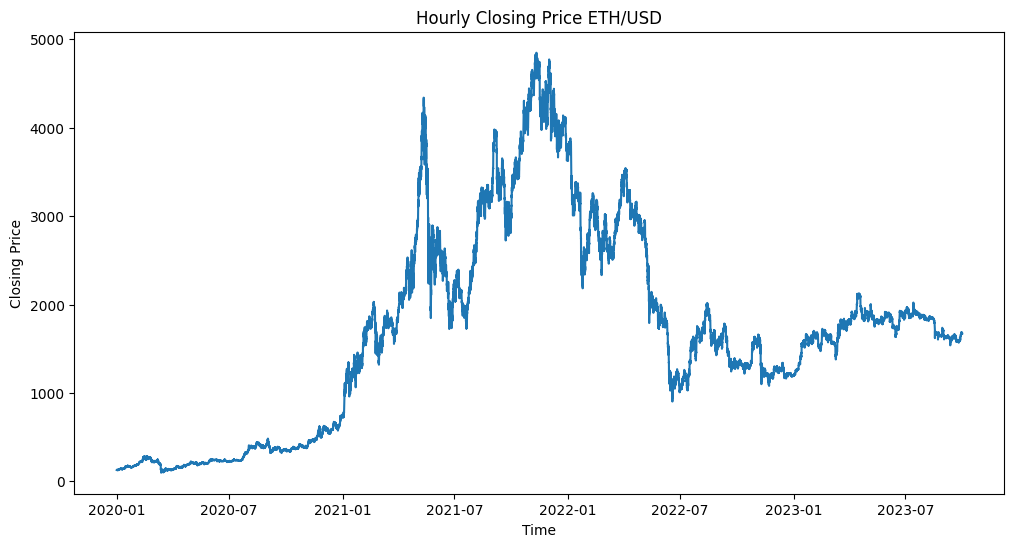
\includegraphics[width=0.93\textwidth]{figures/training_dataset_plot.png}
    \caption{Training Dataset (ETH/USD)}
    \label{fig:training_dataset_plot}
\end{figure}

The created dataset was then used for model tuning (Section \ref{section:model_tuning}), where it was loaded into a Pandas DataFrame. Pandas is a powerful data manipulation and analysis library for Python, which offers an extensive set of tools ideal for manipulating time series data \cite{PandasDocs}, providing a solid foundation for the subsequent feature engineering. 

\subsubsection{Date Time Feature}
\label{section:datetime_feature}

The \texttt{process\_timestamp} function (Listing \ref{lst:process_timestamp}) is designed to perform two key operations on the \texttt{bucket} column of the training dataset:

\begin{enumerate}
    \item \textbf{Conversion to Datetime Objects:}  The function starts by converting the values in the \texttt{bucket} column into datetime objects using the pandas \texttt{to\_datetime()} function. 
    \item \textbf{Handling Missing Data Points (Optional):} Offers an optional feature to handle gaps in the dataset. If the fill parameter is set to True, the function will execute a series of steps to fill in gaps. The dataset is resampled into one-hour intervals using \texttt{data.resample('h').asfreq()}. This step ensures that the time series data is uniformly spaced, creating a consistent time frame for analysis. The function then fills missing values in the \texttt{close\_price} column by carrying forward the last available value (forward fill). This method is chosen as it is a common practice in time series analysis, especially for financial data, where the most recent known value is often the best estimate for missing data. For the \texttt{volume} and \texttt{count} columns, missing values are filled with zeros. This choice reflects the assumption that a lack of data implies no trades or countable events occurred during that time period. 
\end{enumerate}

Finally, the dataset is sorted and reset to ensure that it is ordered correctly and the indices are consistent. \\

\begin{lstlisting}[language=python, caption={Processing timestamp}, label=lst:process_timestamp]
def process_timestamp(data, fill=False): 
    data['bucket'] = pd.to_datetime(data['bucket'])
    data.set_index('bucket', inplace=True)
    if fill: 
        data = data.resample('h').asfreq()
        data['close_price'] = data['close_price'].fillna(method='ffill')
        data['volume'] = data['volume'].fillna(0) 
        data['count'] = data['count'].fillna(0)
    data.sort_values('bucket', inplace=True)
    data.reset_index(inplace=True)
    return data
\end{lstlisting}

After preprocessing the timestamp is split up into hour, day of the week, day of the month, month and year using the \texttt{add\_feature\_date} function (\ref{lst:split_timestamp}. \\

\begin{lstlisting}[language=python, caption={Splitting timestamp}, label=lst:split_timestamp]
def add_feature_date(data):
    # time-based features
    data['hour'] = data['bucket'].dt.hour
    data['day_of_week'] = data['bucket'].dt.dayofweek #Monday=0, Sunday=6
    data['day_of_month'] = data['bucket'].dt.day
    data['month'] = data['bucket'].dt.month
    data['year'] = data['bucket'].dt.year
\end{lstlisting}

The reason for splitting the date and time is because LSTM networks require input features that effectively represent the temporal dynamics in the data. Cyclic encoding is a method used to transform time-related features into a format that preserves their cyclical nature, which is crucial for accurate time series forecasting. The functions \texttt{apply\_cyclic\_encoding} and \texttt{encode\_cyclic\_feature} are instrumental in this process. \\ 
% add a source here to back up why this is good

The \texttt{apply\_cyclic\_encoding} function (Listing \ref{lst:apply_cyclic_encoding}) applies cyclic encoding to specified time-related columns in the dataset. This function takes two parameters: the dataset and a list of columns to apply the encoding to. For each column, it uses the \texttt{get\_distinct\_count} function to determine the length of the cycle (e.g., 24 for hours, 7 for days of the week) and then applies the \texttt{encode\_cyclic\_feature} function to create two new columns for each feature, representing the sine and cosine components of the cyclic encoding.

\begin{lstlisting}[language=python, caption={Applying cyclic encoding}, label=lst:apply_cyclic_encoding]
def apply_cyclic_encoding(data, columms=['hour','day_of_week','month']): 
    for column in columms: 
        cycle_length = get_distinct_count(data, column)
        data[column + "_cos"] = data[column].apply(lambda x: encode_cyclic_feature(x, cycle_length, type='cos')).astype(float)
        data[column + "_sin"] = data[column].apply(lambda x: encode_cyclic_feature(x, cycle_length, type='sin')).astype(float)
    return data
\end{lstlisting}

The \texttt{encode\_cyclic\_feature} function (Listing \ref{lst:encode_cyclic_feature}) takes a single value, the cycle length of the feature, and the type of encoding (sin or cos). It converts the value into radians and then applies either the sine or cosine function. This conversion to a circular format enables the model to recognize that the end of one cycle connects back to the beginning (e.g., the 23rd hour connects back to the 0th hour). The encoding's outcome is illustrated with the \texttt{day\_of\_the\_month} feature, displaying data for the entire year of 2016, as seen in Figure \ref{fig:day_month_encoding}. \\

\begin{lstlisting}[language=python, caption={Encoding cyclic feature}, label=lst:encode_cyclic_feature]
def encode_cyclic_feature(value, cycle_length, type):
    value_rad = (value / cycle_length) * 2 * np.pi
    if type == 'sin':
        return np.sin(value_rad) 
    else: 
        return np.cos(value_rad)
\end{lstlisting}

This encoding is important because for example, hours of the day or days of the week recur in a predictable pattern. By encoding these features as sine and cosine values (Figure \ref{fig:day_month_encoding}), the LSTM can better understand and utilize the periodicity in the data, which in turn should lead to more accurate time series predictions. \\

\textbf{Special Cyclic Encoding for Day of the Month:} \\
The functions \texttt{encode\_day\_of\_month} and \texttt{apply\_day\_of\_month\_encoding} (Listings \ref{lst:encode_day_of_month_feature} \& \ref{lst:apply_day_of_month_feature}) are designed to address the cyclic nature of days in a month, considering the varying lengths of different months. \\

The \texttt{encode\_day\_of\_month} function (Listing \ref{lst:encode_day_of_month_feature}) takes the day of the month, month, and year as inputs and normalizes the day of the month based on the total number of days in a given month. This normalization accounts for the alternating number of days in different months and the edge case of February. The function then applies a cyclic encoding (sine and cosine) to this normalized value. This encoding effectively maps each day to a point on a circle, thus preserving the cyclical pattern of days within a month.

\begin{lstlisting}[language=python, caption={Encoding Day of the Month feature}, label=lst:encode_day_of_month_feature]
def encode_day_of_month(day_of_month, month, year, type):
    normalized_day = (day_of_month - 1) / get_month_length(month, year)  # Subtract 1 to start from 0
    if type == 'sin': 
        return np.sin(2 * np.pi * normalized_day) 
    else: 
        return np.cos(2 * np.pi * normalized_day) 
\end{lstlisting}

The \texttt{apply\_day\_of\_month\_encoding} function (Listing \ref{lst:apply_day_of_month_feature}) applies the \\\texttt{encode\_day\_of\_month} function to each row in the dataset. It adds two new columns, \texttt{day\_of\_month\_sin} and \texttt{day\_of\_month\_cos}, representing the sine and cosine cyclic encoding of the day of the month. This approach ensures that the model recognizes the continuity from the end of one month to the beginning of the next.

\begin{lstlisting}[language=python, caption={Applying Day of the Month Encoding}, label=lst:apply_day_of_month_feature]
def apply_day_of_month_encoding(data): 
    data["day_of_month_sin"] = data.apply(lambda row: encode_day_of_month(row['day_of_month'], row['month'], row['year'], 'sin'), axis=1)
    data["day_of_month_cos"] = data.apply(lambda row: encode_day_of_month(row['day_of_month'], row['month'], row['year'], 'cos'), axis=1)
    return data
\end{lstlisting}

This specialized encoding is crucial for LSTM models that forecast based on date-time data. Standard representations of dates might not effectively convey the cyclic nature of time, particularly for features like the day of the month that do not have a fixed cycle length. By using this cyclic encoding, LSTM models can better capture and utilize the temporal dynamics inherent in the data, leading to potentially more accurate and meaningful predictions, especially in scenarios where the day of the month has a significant impact on the observed time series data (e.g. consumer behavior, financial market trends, etc.). \\

\begin{figure}[H]
    \centering
    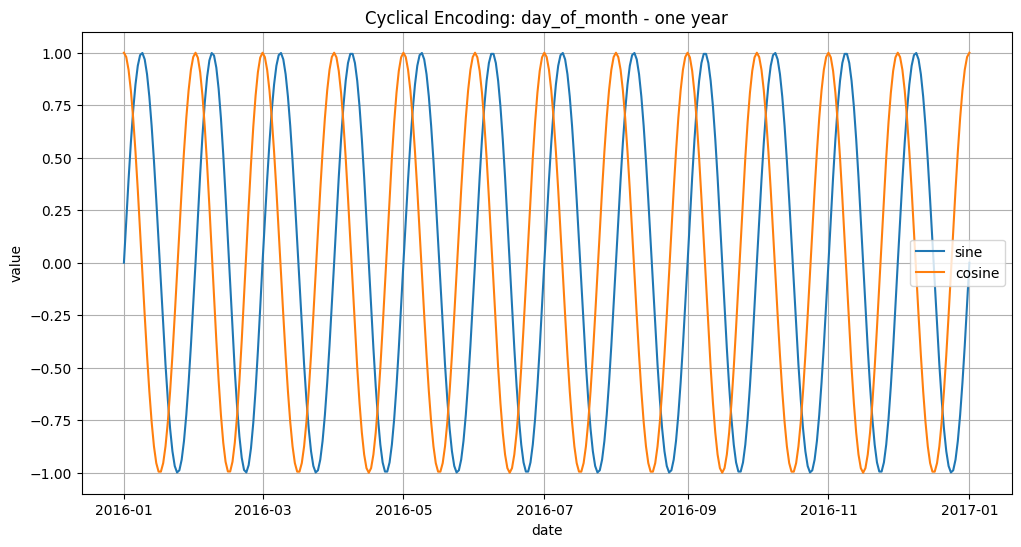
\includegraphics[width=\textwidth]{figures/day_of_the_month_encoding.png}
    \caption{Day of the Month Encoding}
    \label{fig:day_month_encoding}
\end{figure}

\subsubsection{Normalization of the Year Feature}
In time series analysis, particularly when preparing data for LSTM models, normalizing features can be critical to model performance. The function \texttt{normalize\_year} is designed to normalize the \texttt{year} column in the dataset. 
The \texttt{normalize\_year} function (Listing \ref{lst:year_normalization}) takes a dataset and an optional list of column names (defaulting to ['year']). For each specified column, it calculates the minimum and maximum values using the \texttt{get\_min\_max\_value} function. Then, it applies a normalization formula to each value in the column, scaling it to a range between 0 and 1. This normalization is achieved by subtracting the minimum value from the column value and dividing by the range (max - min + 1). The '+1' in the denominator is specifically added to account for the year 2024, ensuring that the scale includes the entire range of years present in the data plus one additional year.

\begin{lstlisting}[language=python, caption={Year normalization}, label=lst:year_normalization]
def normalize_year(data, columns=['year']): 
    for column in columns: 
        min, max = get_min_max_value(data, column)
        data[column+'_normalized'] = data[column].apply(lambda x: normalize_feature(x, min, max+1)) # +1 to account for 2024
    return data
\end{lstlisting}
\mbox{}\\
\paragraph{Importance of Normalization:}
Normalization of the year is crucial for several reasons:
\begin{itemize}
    \item \textbf{Consistency in Scale:} Normalizing ensures that the \texttt{year} feature has a consistent scale compared to other features in the dataset, which is essential for models like LSTMs that are sensitive to the scale of the input data.
    \item \textbf{Improved Model Training:} Features on a similar scale can lead to faster convergence during training, as it helps in maintaining numerical stability and a balanced gradient flow.
\end{itemize}

In summary, the \texttt{normalize\_year} function provides a method to scale the year feature appropriately, enhancing its utility for LSTM models, where scale and continuity of data are key factors for model accuracy and performance.

\subsubsection{US-Holidays Feature}
In the realm of time series forecasting, especially in financial markets, recognizing special calendar events like holidays can be crucial. The function \texttt{add\_holiday\_feature} (Listing \ref{lst:holiday}) is designed to integrate this aspect into the dataset.

\begin{lstlisting}[language=python, caption={US-Holidays feature}, label={lst:holiday}]
def add_holiday_feature(data):
    us_holidays = holidays.UnitedStates()
    data['is_holiday'] = data['bucket'].apply(lambda x: x in us_holidays).astype(int)
    return data
\end{lstlisting}

The \texttt{add\_holiday\_feature} function (Listing \ref{lst:holiday}) introduces a binary feature \\ \texttt{is\_holiday} to the dataset. It utilizes the holidays library to create a list of US holidays and then applies a lambda function to the bucket column, which stores the timestamps. For each timestamp, the function checks whether the date is a US holiday. If so, the \texttt{is\_holiday} column is marked with a 1, otherwise a 0. This binary encoding effectively differentiates regular days from US holidays. 

\paragraph{Potential Impact:}
The inclusion of the \texttt{is\_holiday} feature provides the LSTM model with additional context about the timing of data points. Holidays can impact financial markets in various ways, such as reduced trading volume or closure of markets, which in turn can affect the price movement of assets. By providing this information, the model might be able to better anticipate and account for these irregularities in the data.
However, it is important to consider the global nature of cryptocurrency trading when evaluating the impact of this feature. The \texttt{ETH/USD} market, like other cryptocurrency markets, operates worldwide and is not confined to a single timezone or region. Therefore, while US holidays might have some influence, their impact could be less pronounced compared to traditional markets that are more regionally focused. This means that while the \texttt{is\_holiday} feature could contribute to the model's understanding of certain market behaviors, its overall influence on a global and decentralized market like \texttt{ETH/USD} might be overvalued.

\subsubsection{Logarithmic Scaling}

Applying appropriate transformations to the input features is crucial for optimizing the performance of LSTM models in time series analysis. The \texttt{apply\_log\_scaler} function is designed to apply a logarithmic transformation to specific features in the dataset. \\

The \texttt{apply\_log\_scaler} function (Listing \ref{lst:log_scaler}) takes a dataset and a list of column names (defaulting to ['close\_price', 'volume', 'close\_lag12', 'close\_lag168']). For each column in this list, it applies the natural logarithm transformation using the \texttt{np.log1p} (numpy) function. This function computes the natural logarithm of one plus the input value, effectively scaling the data while also handling zero values gracefully. \\

\begin{lstlisting}[language=python, caption={Logarithmic Scaling Function}, label=lst:log_scaler]
def apply_log_scaler(data, columns=['close_price', 'volume', 'close_lag12', 'close_lag168']): 
    for column in columns:
        data[column] = np.log1p(data[column])
    return data
\end{lstlisting}

\paragraph{Importance of Logarithmic Scaling}
Logarithmic scaling is particularly beneficial in time series forecasting for several reasons:
\begin{itemize}
    \item \textbf{Handling Skewed Data:} A lot of financial time series data, like prices and volumes, can be highly skewed. Logarithmic scaling helps in reducing this skewness, making the data distribution more symmetrical and thus more suitable for LSTM models.
    \item \textbf{Stabilizing Variance:} This transformation tends to stabilize the variance across the data, which can be highly beneficial for models that assume constant variance in the input features.
    \item \textbf{Multiplicative to Additive:} Converts multiplicative relationships into additive ones, which can be easier for models like LSTMs to learn and capture in their predictions.
\end{itemize}

\paragraph{Selection of Features:}
The choice of features for logarithmic scaling (eg.: 'close\_price', 'volume', 'close\_lag12', 'close\_lag168', 'count') is based on their characteristics in financial time series data. These features often exhibit exponential growth or decay, and logarithmic scaling can transform them into a more linear relationship. This can be beneficial for the learning process of LSTM networks. \\

In conclusion, the \texttt{apply\_log\_scaler} function plays a vital role in preprocessing the data for LSTM models, particularly in financial time series analysis, by transforming key features to a form that is more conducive to the learning and predictive capabilities of these models.

\subsubsection{Lag Feature}

Lag features are a critical component in time series forecasting, particularly when using LSTM models that are designed to capture temporal dependencies. The \texttt{add\_feature\_lag} function adds these lag features to the dataset, enhancing the model's ability to learn from past data. \newline

The \texttt{add\_feature\_lag} function (Listing \ref{lst:lag_feature}) takes a dataset and a list of integers representing the lags to be created. For each lag in the list it creates a new column in the dataset, labeled \texttt{close\_lag} followed by the lag number. This new column contains the close\_price feature shifted by the number of time steps specified by the lag. This shift means that each new \texttt{close\_lagX} column contains the close\_price from X time steps in the past.

\begin{lstlisting}[language=python, caption={Lag Feature}, label=lst:lag_feature]
def add_feature_lag(data, lags=[1]): 
    for lag in lags: 
        data['close_lag'+str(lag)] = data['close_price'].shift(lag)
    return data
\end{lstlisting}

\paragraph{Importance of Lag Features}
Lag features are vital in time series analysis for several reasons:
\begin{itemize}
    \item \textbf{Capturing Temporal Dependencies:} They allow the model to access past values of the time series, which is essential for capturing patterns and trends over time.
    \item \textbf{Enhancing Forecast Accuracy:} By providing the model with historical data points, lag features can significantly improve the accuracy of forecasts.
    \item \textbf{Flexibility in Model Design:} Different lags can capture different aspects of temporal dynamics, allowing for a more nuanced and comprehensive model.
\end{itemize}

In summary, the \texttt{add\_feature\_lag} function provides a simple yet powerful way to enrich a time series dataset with past information, enabling LSTM models to make more informed predictions.

\subsubsection{Moving Averages}

Moving averages are a foundational tool in time series analysis, particularly in financial markets where they help in identifying trends and smoothing out short-term fluctuations. The functions \texttt{simple\_moving\_average} and \texttt{exponential\_moving\_average} add these moving average features to the dataset. \\

The \texttt{simple\_moving\_average} function (Listing \ref{lst:sma}) computes the simple moving average (SMA) for specified columns over given window sizes. For each column and window size, it creates a new column in the dataset labeled \texttt{sma\_WINDOWSIZE\_COLUMN}, where \texttt{WINDOWSIZE} is the size of the moving window, and \texttt{COLUMN} is the name of the original column. The SMA is calculated by averaging the values of the column over the specified window size. \\

Similarly, the \texttt{exponential\_moving\_average} function (Listing \ref{lst:ema}) calculates the exponential moving average (EMA) for the specified columns. EMA gives more weight to recent data points, making it more responsive to new information. For each column and span size, it adds a new column labeled \texttt{ema\_SPAN\_COLUMN}. The span size determines the rate at which older observations are weighted down. \\

\begin{lstlisting}[language=python, caption={Simple Moving Average Feature}, label={lst:sma}]
def simple_moving_average(data, window_sizes, columns=['close_price']): 
    for column in columns: 
        for window_size in window_sizes: 
            data['sma_'+str(window_size)+"_"+column] = data[column].rolling(window=window_size).mean()
    return data
\end{lstlisting}

\begin{lstlisting}[language=python, caption={Exponential Moving Average Feature}, label={lst:ema}]
def exponential_moving_average(data, span_sizes,columns=['close_price']):
    for column in columns: 
        for span in span_sizes: 
            data['ema_'+str(span)+"_"+column] = data[column].ewm(span=span).mean()
    return data
\end{lstlisting}

\paragraph{Importance of Moving Averages}
Moving averages are especially useful in the context of LSTM models for several reasons:
\begin{itemize}
    \item \textbf{Data Smoothing:} They help in smoothing out random fluctuations in the data, highlighting underlying trends, which can be beneficial for LSTMs in capturing long-term dependencies.
    \item \textbf{Trend Identification:} Moving averages can assist the model in identifying and adapting to trends in the data, which is vital in forecasting tasks.
    \item \textbf{Re-activeness to Recent Changes:} EMAs can provide a more reactive feature that responds quickly to recent changes in the data, potentially improving the model's ability to predict short-term movements.
\end{itemize}

\paragraph{Application in Financial Time Series:}
In financial time series forecasting, such as stock or cryptocurrency prices, moving averages are instrumental in understanding market behavior. They can act as indicators of potential support and resistance levels, trend directions, and momentum, which can be crucial inputs for an LSTM model aiming to predict future price movements.

In conclusion, the \texttt{simple\_moving\_average} and \texttt{exponential\_moving\_average} functions enrich the dataset with essential trend-based features, enhancing the predictive capabilities of LSTM models in time series analysis.

% dataset: https://support.kraken.com/hc/en-us/articles/360047543791-Downloadable-historical-market-data-time-and-sales-

\subsection{Model Tuning}
\label{section:model_tuning}

Effective model tuning is pivotal in the development of robust and accurate forecasting models. This section delves into the intricate process of fine-tuning the Long Short-Term Memory (LSTM) network, specifically tailored for time series forecasting of the \texttt{ETH/USD} currency pair. The focus is on leveraging a comprehensive parameter grid to systematically explore a multitude of feature combinations and model configurations. This systematic approach ensures a thorough exploration of the parameter space, leading to an optimized model that can effectively capture the complexities of the time series data. \\

Central to this process is the utilization of MLflow, a versatile platform for managing the machine learning lifecycle, including experimentation, reproducibility, and deployment. MLflow plays a critical role in tracking experiments, enabling an organized and efficient review of model performance across different configurations. The ability to log and compare various parameters, metrics, and models streamlines the model selection process and fosters a methodical approach to model tuning. \\

\subsubsection{Setting Up the Model Tuning Environment}

The model tuning process is orchestrated within a Jupyter Notebook, which serves as an interactive computational environment for running the tuning script. This setup not only facilitates an intuitive and flexible way to run complex analyses but also allows for immediate visualization and interaction with the data and models. \\

A crucial aspect of this setup is the integration with various services, managed through Docker containers, to streamline the model tracking and data storage processes. The Jupyter Notebook is configured to interact with the following services. \\

\begin{itemize}
    \item \textbf{MLflow Docker Container:} The MLflow tracking server is set up in a Docker container (Section \ref{section:mlflow_docker}). By setting the MLflow tracking URI to \url{http://127.0.0.1:5000}, the Jupyter Notebook connects to the MLflow server running locally within the Docker container. This connection allows for the systematic tracking of experiments, including logging parameters, metrics, and models.

    \item \textbf{MinIO Docker Container:} MinIO (Section \ref{section:minio}) is utilized for storing artifacts related to the machine learning experiments. The Jupyter Notebook is configured to interact with the MinIO server through specified AWS credentials and the S3 endpoint URL. The AWS credentials \texttt{AWS\_ACCESS\_KEY\_ID} and \texttt{AWS\_SECRET\_ACCESS\_KEY} are set as environment variables. Additionally, the \texttt{MLFLOW\_S3\_ENDPOINT\_URL} environment variable is set to the MinIO server's address, \url{http://172.1.0.12:2000}, enabling the storage and retrieval of MLflow artifacts within the MinIO storage.

    \item \textbf{PostgreSQL Database:} PostgreSQL (Section \ref{section:timescale_docker}) is employed to store model tracking information. The integration with PostgreSQL allows for efficient management and querying of experiment data, enhancing the ability to analyze and compare different model versions and configurations.
\end{itemize}

This environment setup provides a robust and scalable framework for model tuning, ensuring that all aspects of the machine learning process, from experiment tracking to artifact storage, are meticulously managed and easily accessible.\\

\begin{lstlisting}[language=python, caption={Model Tuning Evnironment Setup}, label={lst:model_tuning_environment}]
os.environ["AWS_ACCESS_KEY_ID"] = "eITEO5kyE7hccuy7UTHv"
os.environ["AWS_SECRET_ACCESS_KEY"] = 
    "5KBCscit30Z70bSVGIMvMBBoqV8ydn232o2MW9RA"
os.environ["MLFLOW_S3_ENDPOINT_URL"] = f"http://172.1.0.12:2000"

mlflow.set_tracking_uri(uri="http://127.0.0.1:5000")
\end{lstlisting}

\subsubsection{Construction of the Parameter Grid}

In the model tuning phase, a comprehensive parameter grid is constructed to systematically evaluate different combinations of features and LSTM model hyperparameters, which is essential to optimize the model's performance.

\paragraph{Feature Combinations}
The parameter grid begins with the specification of fixed and optional features. Fixed features include essential time-related attributes like 'hour', 'day of week', 'month', 'day of month', normalized 'year', as well as other relevant features such as 'is\_holiday', 'volume', 'is\_weekend', 'count', and 'close\_price'. These features are considered crucial for capturing the fundamental temporal patterns in the time series data. \\

\begin{lstlisting}[language=python, caption={Model Tuning Fixed and Optional Features}, label={lst:model_tuning_fixed_optional_features}]
fixed_features = ['hour_cos', 'hour_sin', 'day_of_week_cos',
    'day_of_week_sin', 'month_cos', 'month_sin',
    'day_of_month_sin', 'day_of_month_cos', 'year_normalized',
    'is_holiday', 'volume', 'is_weekend', 'count', 'close_price']
    
optional_features = ['close_lag12','close_lag6', 'close_lag168',
    'sma_6_close_price', 'ema_6_close_price', 'ema_12_close_price' ]

# generating all combinations of optional features
all_feature_combinations = []
for r in range(len(optional_features) + 1):
    for subset in itertools.combinations(optional_features, r):
        all_feature_combinations.append(fixed_features + list(subset))

print(len(all_feature_combinations))
\end{lstlisting}
In addition to these fixed features, a set of optional features are defined. These include various lagged values of the closing price (e.g. 'close\_lag12', 'close\_lag6', 'close\_lag168'), simple and exponential moving averages (e.g. 'sma\_6\_close\_price', 'ema\_6\_close\_price', 'ema\_12\_close\_price'). These optional features are intended to capture more nuanced trends and dependencies in the data. \\

A key step in the grid setup involves generating all possible combinations of these optional features using Python's \texttt{itertools.combinations} (Listing \ref{lst:model_tuning_fixed_optional_features}). This ensures that every subset of the optional features, from empty to the full set, is considered, allowing for a thorough exploration of the feature space.

\begin{lstlisting}[language=python, caption={Model Tuning Parameter Grid}, label={lst:model_tuning_parameter_grid}]
param_grid = {
    'features': all_feature_combinations,
    'lookback': [12,16,24],
    'learning_rate': [0.01, 0.001],
    'optimizer': ['adam', 'adagrad'],
    'batch_size': [8,16,32,64],
    'datatype': [np.float16, np.float32],
    'epochs': [75],
    'loss': ['mean_squared_error'],
    'metrics' : [['mean_absolute_error', 'mean_squared_error', 'accuracy']]
    # double list to not alternate between the metrics
}
grid = ParameterGrid(param_grid)
\end{lstlisting}

\paragraph{Hyperparameter Settings}
The parameter grid (Listing \ref{lst:model_tuning_parameter_grid}) includes a range of hyperparameters for the LSTM model. These hyperparameters include:
\begin{itemize}
    \item \textbf{Lookback}: Defines the number of previous time steps to use as input variables. For instance, a lookback of 12 indicates that the model uses data from the past 12 time units for forecasting.
    \item \textbf{Learning Rate}: The step size at each iteration while moving toward a minimum of a loss function.
    \item \textbf{Optimizer}: Sets the method used for updating weights in the network.
    \item \textbf{Batch Size}: Number of samples processed before the model is updated.
    \item \textbf{Datatype}: Defines the data type used for the model, with np.float32 being a common choice for neural network computations.
    \item \textbf{Epochs}: Complete passes through the training dataset.
    \item \textbf{Loss Function}: Evaluating the model's prediction accuracy.
    \item \textbf{Metrics}: Additional metrics for evaluating the model's performance, including 'mean\_absolute\_error', 'mean\_squared\_error', and 'accuracy'.
\end{itemize}

The \texttt{ParameterGrid} from Python's scikit-learn library \cite{ScikitLearnParameterGrid} is utilized to generate a grid of all combinations of these features and hyperparameters. The length of the grid indicates the total number of different configurations that will be evaluated during the model tuning process.  For this configuration '6144' combinations would be evaluated, but evaluating all these combinations in the model tuning process is a demanding endeavor, requiring significant computational resources and time, and therefore might not be feasible. \\

Through this extensive parameter grid, the tuning script is equipped to conduct a detailed and exhaustive search for the optimal model configuration, balancing the richness of features with the model's complexity and performance.

\subsubsection{Data Preparation Function}
The \texttt{data\_prep} function (Listing \ref{lst:model_tuning_data_prep}) encapsulates a series of data pre-processing steps, which have been outlined in the Section \ref{section:data_preparation} and are crucial for molding the raw dataset into a format suitable for LSTM training. \\  

The function begins by removing certain columns deemed unnecessary for the model, specifically open-, high-, and low price. This step focuses the dataset on the most relevant features for forecasting. Next, the \texttt{process\_timestamp} function is applied (see \ref{section:datetime_feature}). \\

Several functions are then used to add new features and apply encodings as outlined earlier:
\begin{itemize}
    \item \texttt{add\_feature\_date} enriches the dataset with date-related features.
    \item \texttt{add\_holiday\_feature} marks US holidays in the dataset, providing additional context that may influence market behavior.
    \item \texttt{apply\_cyclic\_encoding} and \texttt{apply\_day\_of\_month\_encoding} are used to encode time-related features such as hour, day\_of\_week, and month cyclically.
    \item \texttt{normalize\_year} normalizes the year feature, scaling it appropriately for the LSTM model.
\end{itemize}

Further transformations are applied to the data:
\begin{itemize}
    \item The true close\_price is preserved in a new column close\_price\_true before transformations.
    \item \texttt{apply\_log\_scaler} is used to logarithmically scale features like close\_price, volume, and count, stabilizing their variance and reducing skewness.
    \item \texttt{add\_feature\_lag} introduces lag features, providing the model with historical data points.
    \item \texttt{simple\_moving\_average} and \texttt{exponential\_moving\_average} compute moving averages of the close\_price, capturing trends over different time horizons.
\end{itemize}

Finally, columns that are no longer needed, such as symbol\_id, hour, day\_of\_week, day\_of\_month, month and year, are dropped because their information is now encoded in other features. The function concludes by dropping any NaN values, ensuring the dataset is clean and consistent. \\

The \texttt{data\_prep} function is integral to transforming the raw time series data into a rich, feature-enhanced format ready for LSTM modeling. Each step is methodically designed to extract and encode meaningful patterns from the dataset, providing a solid foundation for accurate and insightful time series forecasting (Section \ref{section:model_dev}).

\begin{lstlisting}[language=python, caption={Model Tuning Data Preperation}, label={lst:model_tuning_data_prep}]
def data_prep(data):
    data = data.drop(columns=['open_price', 'high', 'low'], axis=1)
    data = process_timestamp(data, fill=True)
    data = add_feature_date(data)
    data = add_holiday_feature(data)
    data = apply_cyclic_encoding(data, columms=['hour', 'day_of_week', 'month'])
    data = apply_day_of_month_encoding(data)
    data = normalize_year(data) # has to be updated yearly (because of the min-max scaler - max+1 is currently set = 2024)
    data['close_price_true'] = data['close_price'] # save the true price --> for unseen data plot
    data = apply_log_scaler(data, columns=['close_price', 'volume', 'count'])
    data = add_feature_lag(data, lags=[1,4,6,12,24,168])
    data = simple_moving_average(data, window_sizes=[6,12,168], columns=['close_price']) # window sizes are in hours
    data = exponential_moving_average(data, span_sizes=[6,12,24,96,168], columns=['close_price']) # span sizes are in hours
    # not needed as these values are encoded to be cyclic 
    data = data.drop(columns=['symbol_id', 'hour', 'day_of_week', 'day_of_month', 'month', 'year'], axis=1)
    # dropping nan values which are created because of simple_moving_average and lags 
    data = data.dropna()
    return data
\end{lstlisting}


\subsubsection{Loading and Pre-processing the Dataset}
Initially, the raw dataset is loaded from a CSV file, \texttt{ETHUSD.csv}, into a Pandas DataFrame (Listing \ref{lst:model_tuning_data_load}). This DataFrame, \texttt{raw\_data}, contains the unprocessed OHLC time series data for the \texttt{ETH/USD} currency pair. The \texttt{data\_prep} function is then applied to this raw dataset, performing a series of pre-processing steps as previously outlined. The output, stored in the \texttt{data} DataFrame, represents the processed and feature-engineered dataset, ready for use in model training and evaluation.

\paragraph{Splitting the Dataset}
\label{section:splitting_dataset}
In the next step, the dataset is split into training and testing subsets (Listing \ref{lst:model_tuning_data_load}). This split is crucial for validating the model's performance on unseen data and ensuring that it generalizes well beyond the data it was trained on. 
\begin{itemize}
    \item The \texttt{test} subset consists of the last 1\% of the data and this portion is set aside to evaluate the model's performance after training. The choice of the last 1\% of the dataset ensures that the test set is representative of the most recent patterns in the data, which is often critical in time series forecasting.
    \item The \texttt{training} subset contains the remaining 99\% of the data. This larger portion is used to train the models.
\end{itemize}

\begin{lstlisting}[language=python, caption={Model Tuning Loading and Splitting the Dataset}, label={lst:model_tuning_data_load}]
# Prep data once for all models: 
file_path = 'ETHUSD.csv'
raw_data = pd.read_csv(file_path)
data = data_prep(raw_data)

test = data.iloc[int(len(data)*0.99):] 
training = data.iloc[:int(len(data)*0.99)]
training.head()
\end{lstlisting}

\paragraph{Previewing the Training Data}
Finally, the \texttt{head()} method is called on the \texttt{training} DataFrame to preview the first few rows of the training dataset. This step is a standard practice in data analysis, providing a quick snapshot of the dataset's structure and the pre-processing outcomes, ensuring that the data is correctly formatted and ready for the subsequent model tuning process.

In summary, this segment of the code is foundational for setting up the modeling phase. It ensures that the data is not only pre-processed and feature-enriched but also appropriately partitioned into training and testing sets, paving the way for effective and reliable model development and evaluation.

\subsubsection{Model Tuning Routine}

The model tuning routine is a systematic approach to training and evaluating the LSTM model across a range of parameters, which is integral to identifying the optimal model configuration for forecasting the \texttt{ETH/USD} currency pair.

\paragraph{Initialization and Early Stopping}
Before the routine is started a run counter and an early stopping mechanism is initialized (Listing \ref{lst:model_tuning_early_stop}). The early stopping callback is used to halt the training process if the model ceases to show improvement, thereby preventing unnecessary processing time.

\begin{lstlisting}[language=python, caption={Model Tuning Early Stoppping}, label={lst:model_tuning_early_stop}]
run_count = 0
early_stopping = EarlyStopping(monitor='loss', min_delta=0.005, patience=10, verbose=1, mode='min')
\end{lstlisting}

\paragraph{Iterating over the Parameter Grid}
The core of the tuning routine is iterating over the parameter grid, which contains all possible combinations of features and hyperparameters. For each set of parameters in the grid:
\begin{enumerate}
\item A new MLflow run is initiated to track the experiment details, and the current set of parameters and data sizes are logged in MLflow for traceability (Listing \ref{lst:model_tuning_main_loop}).

\begin{lstlisting}[language=python, caption={Model Tuning Main Loop}, label={lst:model_tuning_main_loop}]
for params in grid:
    with mlflow.start_run():
        clear_output(wait=True)
        print(run_count)
        # log the currently used parameters
        mlflow.log_params(params)

        # logging training size 
        mlflow.log_param("training data size", len(training))
        mlflow.log_param("unseen test data size", len(test))
\end{lstlisting}
    
\item The LSTM model is configured based on the parameters, including the lookback period, selected features, and layer configuration. The model's architecture, such as the number of units in LSTM and dropout layers, is dynamically adjusted according to the parameters (Listing \ref{lst:model_tuning_lstm_layers}) or could be statically defined to be the same for all iterations.
    
\begin{lstlisting}[language=python, caption={Model Tuning Setting up the LSTM Layers}, label={lst:model_tuning_lstm_layers}]
lookback = params['lookback']
features = params['features']
n_features = len(features)           

model_layers_config = [
    {'type': 'LSTM', 'units': lookback * n_features, 'return_sequences': True, 'input_shape': (lookback, n_features)},  
    {'type': 'LSTM', 'units': lookback * n_features, 'return_sequences': True},  
    {'type': 'LSTM', 'units': lookback * n_features, 'return_sequences': False},      
    {'type': 'Dense', 'units': 1, 'activation': 'selu'}
]

mlflow.log_param("model_layers_config", model_layers_config)

model = create_lstm_model(model_layers_config)
model.compile(optimizer=Adam(learning_rate=params['learning_rate']), loss=params['loss'], metrics=params['metrics'])
\end{lstlisting}


\item The dataset is transformed into sequences suitable for LSTM input, considering the specified lookback period and features. Following this step, the data is split into training and validation sets, with the validation set comprising the latter part of the data (Listing \ref{lst:model_tuning_data_splitting}).

\begin{lstlisting}[language=python, caption={Model Tuning Splitting Dataset into Traning \& Validation}, label={lst:model_tuning_data_splitting}]
# prep data
X, y = create_sequences_np(data=training, features=features, lookback=lookback, datatype=params['datatype'])

training_validation_split = 0.8
split_idx = int(len(X) * training_validation_split)

mlflow.log_param("training_validation_split", training_validation_split)

# validation set with the last 20 percent of the dataset 
X_train, X_val = X[:split_idx], X[split_idx:]
y_train, y_val = y[:split_idx], y[split_idx:]

mlflow.log_param("X_train.shape", X_train.shape)
mlflow.log_param("y_train.shape", y_train.shape)

mlflow.log_param("X_val.shape", X_val.shape)
mlflow.log_param("y_val.shape", y_val.shape)
\end{lstlisting}

\item The model is trained using the training set, with the validation data providing the evaluation of the current performance during training. At the end of the run a plot is created showing the models performance on the validation set, which is saved using MlFlow for the evaluation (Listing \ref{lst:model_tuning_training_validation}).

\begin{lstlisting}[language=python, caption={Model Tuning Traning and Validation}, label={lst:model_tuning_training_validation}]
# train model
model.fit(X_train, y_train, epochs=params['epochs'], batch_size=params['batch_size'], validation_data=(X_val, y_val), callbacks=[early_stopping]) 

# Evaluate your model
# Validation Data
y_pred = model.predict(X_val)

y_val_true = np.expm1(y_val)
y_pred_true = np.expm1(y_pred)

fig, ax = plt.subplots(figsize=(15, 7))
ax.plot(y_val_true, label='Actual Values')
ax.plot(y_pred_true, label='Predicted Values')
ax.set_title('LSTM Model Validation Plot')
ax.set_xlabel('Time')
ax.set_ylabel('Close Price')
ax.set_yscale('log')
ax.legend()
fig.tight_layout()
artifact_path = 'plots'
mlflow.log_figure(fig, artifact_path + '/validation_plot.png')
plt.close(fig)
\end{lstlisting}

\item The model is tested by generating predictions on unseen data. Predicted and actual prices are then plotted against time to visualize the model's performance on data it has not been trained on. The plot is saved using MlFlow. (Listing \ref{lst:model_tuning_unseen_data})

\begin{lstlisting}[language=python, caption={Model Tuning Unseen Data}, label={lst:model_tuning_unseen_data}]
# Unseen Data
predicted_prices = []
actual_prices = test['close_price_true'].values[lookback:] #prices (not log) 
timestamps = test['bucket'].values[lookback:] #timestamps

for i in range(lookback, len(test)):
    last_sequence = test.iloc[i-lookback:i][features].values.reshape((1, lookback, len(features)))
    last_sequence = np.array(last_sequence).astype(np.float16)
    predicted_log_price = model.predict(last_sequence)
    predicted_price = np.expm1(predicted_log_price)[0, 0] # inverse log
    predicted_prices.append(predicted_price)
    
predicted_prices = np.array(predicted_prices)

fig, ax = plt.subplots(figsize=(15, 7))
ax.plot(timestamps, actual_prices, label='Actual Prices', color='blue')
ax.plot(timestamps, predicted_prices, label='Predicted Prices', color='orange')
ax.set_title('LSTM Model Predictions vs Actual Prices')
ax.set_xlabel('Date/Time')
ax.set_ylabel('Close Price')
labels = ax.get_xticklabels()
#ax.set_xticklabels(labels, rotation=45)
ax.legend()
fig.tight_layout()
artifact_path = 'plots'
mlflow.log_figure(fig, artifact_path + '/unseen_test_plot.png')
plt.close(fig)
\end{lstlisting}


\item Several performance metrics, such as mean squared error (MSE), mean absolute error (MAE), root mean squared error (RMSE), mean absolute percentage error (MAPE), R-squared value, and explained variance are calculated and logged in MLflow. These metrics provide a quantitative assessment of the model’s accuracy and reliability. Additionally, the trained model is logged in MLflow, enabling easy retrieval and deployment (Listing \ref{lst:model_tuning_metrics}).

\begin{lstlisting}[language=python, caption={Model Tuning Metrics}, label={lst:model_tuning_metrics}]
# calculate some metrics 
mse_value = mean_squared_error(actual_prices, predicted_prices)
mae_value = mean_absolute_error(actual_prices, predicted_prices)
rmse_value = np.sqrt(mse_value)
mape_value = np.mean(np.abs((actual_prices - predicted_prices) / actual_prices)) * 100
r2_value = r2_score(actual_prices, predicted_prices)
explained_variance = explained_variance_score(actual_prices, predicted_prices)

mlflow.log_metric('mse', mse_value)
mlflow.log_metric('mae', mae_value)
mlflow.log_metric('rmse', rmse_value)
mlflow.log_metric('mape', mape_value)
mlflow.log_metric('r2', r2_value)
mlflow.log_metric('explained_variance', explained_variance)

mlflow.sklearn.log_model(model, "model")

run_count = run_count + 1
\end{lstlisting}
\end{enumerate}

\subsubsection{Overview of MLflow Model Tuning Results}
Throughout the model tuning process, MLflow serves as a centralized platform for monitoring, evaluating, and comparing the performance of various LSTM models.
The MLflow Experiments dashboard (Figure \ref{fig:mlflow_overview}) provides an overview of all the runs conducted during the tuning process. It highlights various runs with unique identifiers and provides a summary of their performance metrics, allowing for an at-a-glance evaluation of which models are performing well according to the chosen criteria. The dashboard enables quick navigation through different runs, facilitating an efficient workflow for identifying the best-performing models. \\

\textbf{MLflow Model Parameters, Architecture and Metrics}
After selecting one of the models from the overview a more detailed view (Figure \ref{fig:mlflow_parameter}) of the model parameters and configuration of the trained model can be viewed. It lists the hyperparameters used in the run, such as batch size, data types, epochs, features selected, learning rate, lookback window, and the specific loss function. Additionally, it includes the model's architecture details, showing the layer configuration with units, activation functions, and other architectural choices. This detailed parameter logging is essential for reproducibility and systematic analysis of the models performance. \\

\begin{figure}[H]
    \centering
    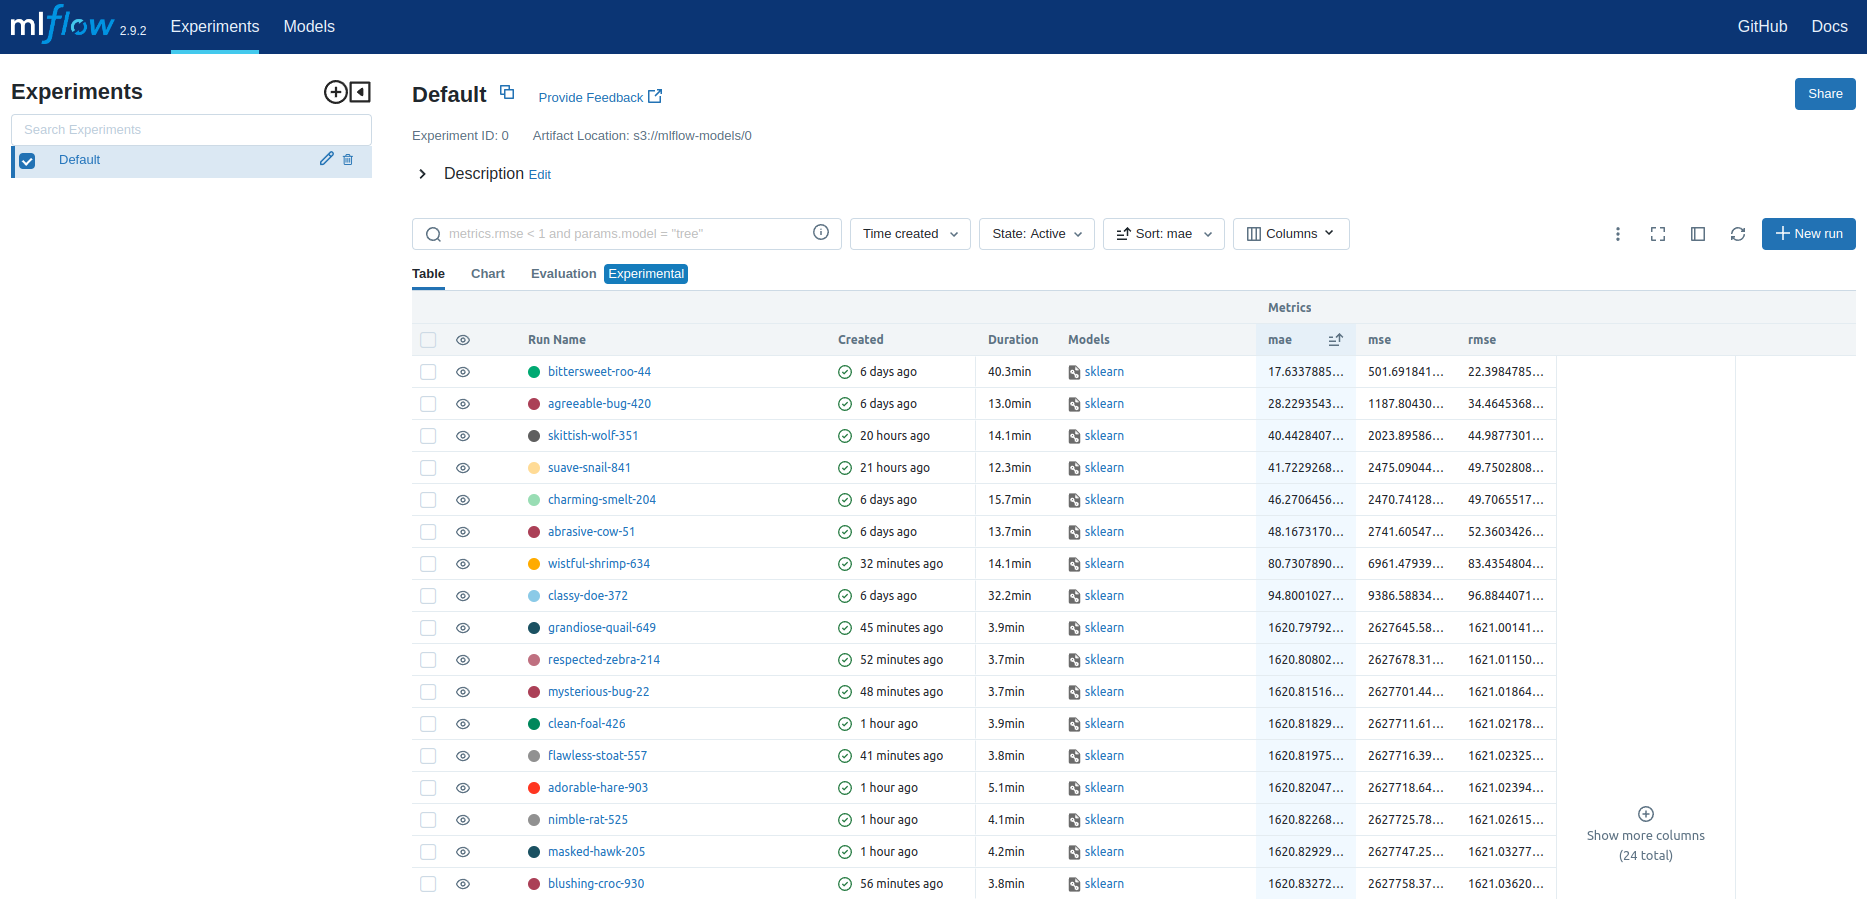
\includegraphics[width=\textwidth]{figures/MLFlow_Model_Overview.png}
    \caption{MlFlow Overview}
    \label{fig:mlflow_overview}
\end{figure}

\begin{figure}[H]
    \centering
    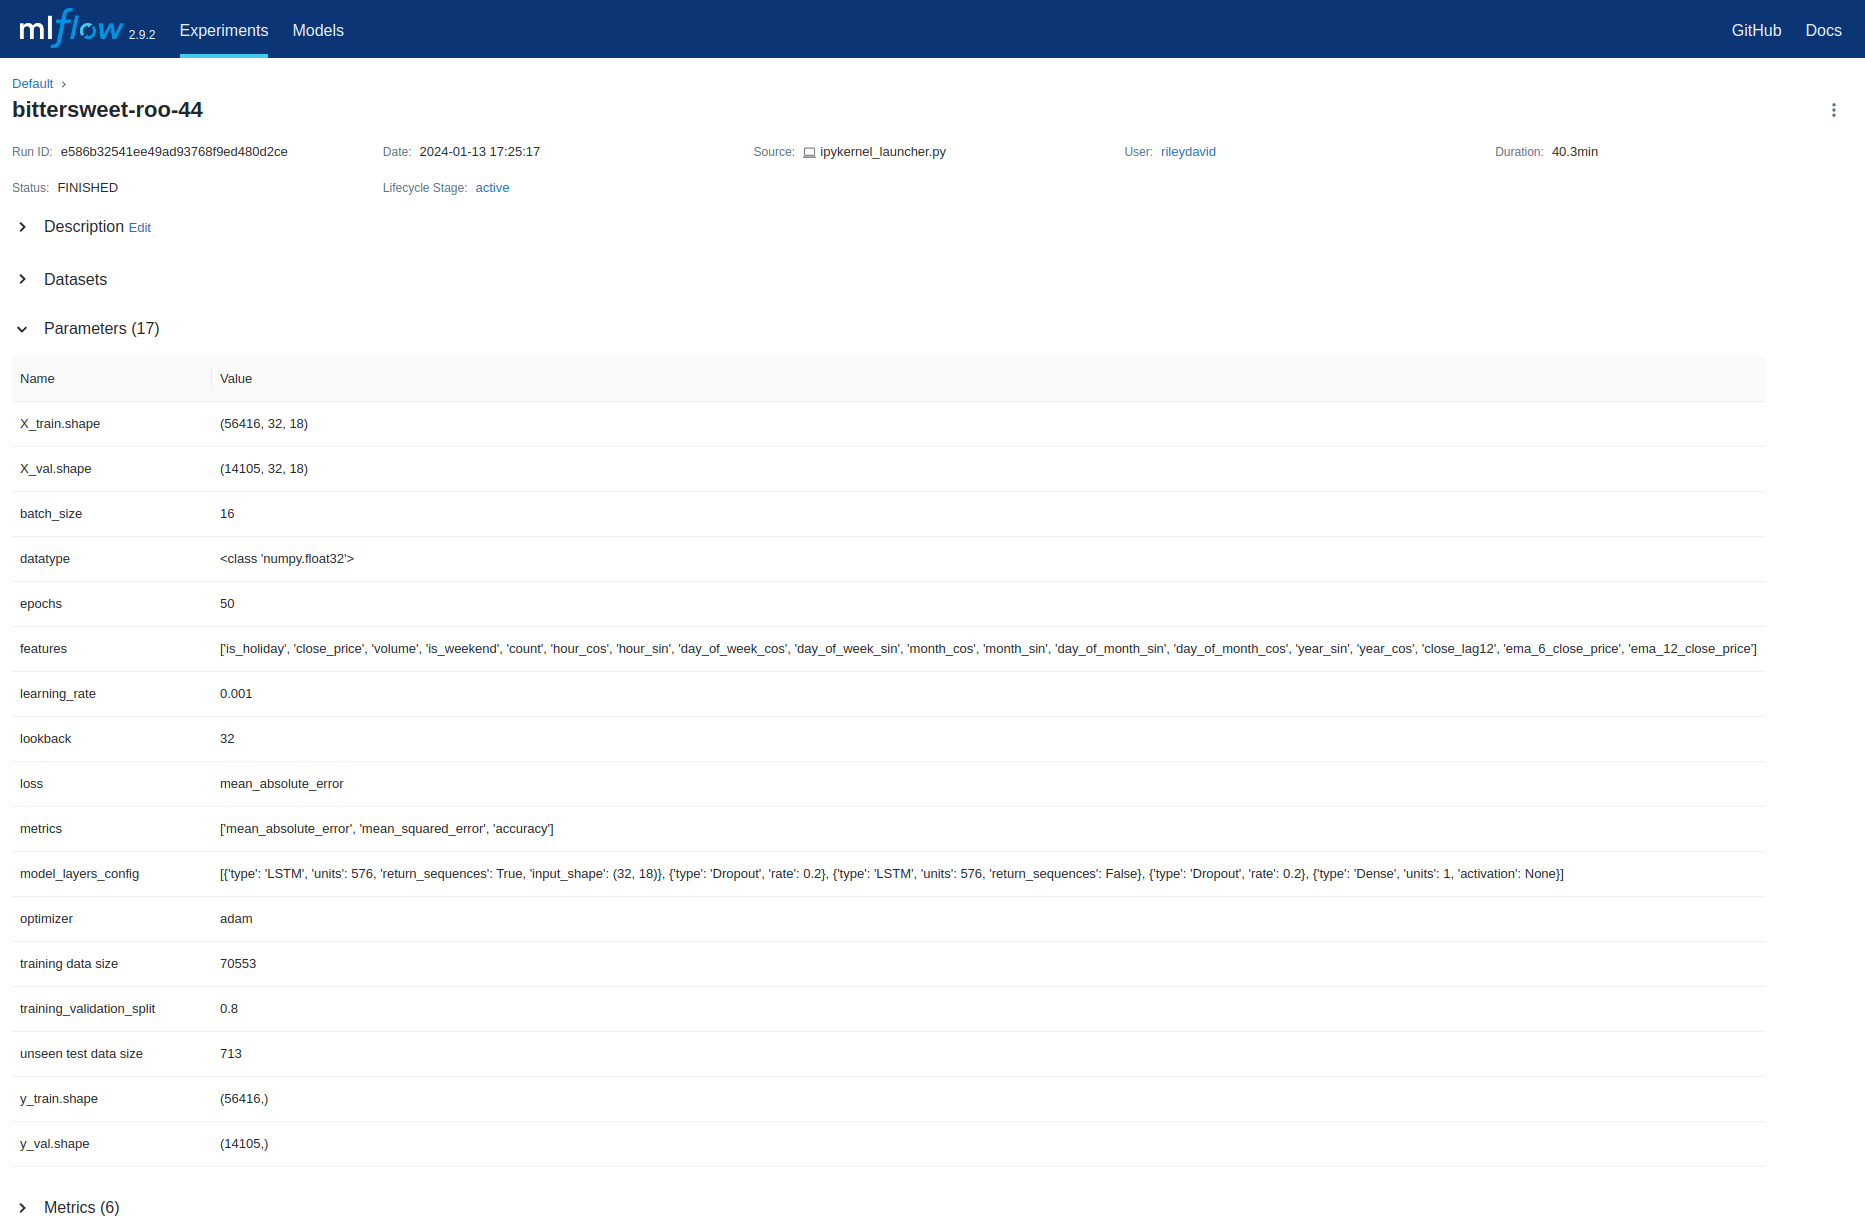
\includegraphics[width=0.93\textwidth]{figures/MlFlow_Model_parameters.png}
    \caption{MlFlow Parameter Tracking}
    \label{fig:mlflow_parameter}
\end{figure}

This provides the user with an overview of the metrics (Figure \ref{fig:mlflow_metrics}) from an MLflow run. The interface displays the metrics recorded for a specific model, such as explained variance, mean absolute error (MAE), mean absolute percentage error (MAPE), mean squared error (MSE), R-squared (r2), and root mean squared error (RMSE). These metrics are critical for assessing the model's predictive accuracy and variance explanation capability. The values are neatly tabulated, allowing for quick review and comparison. 

\begin{figure}[H]
    \centering
    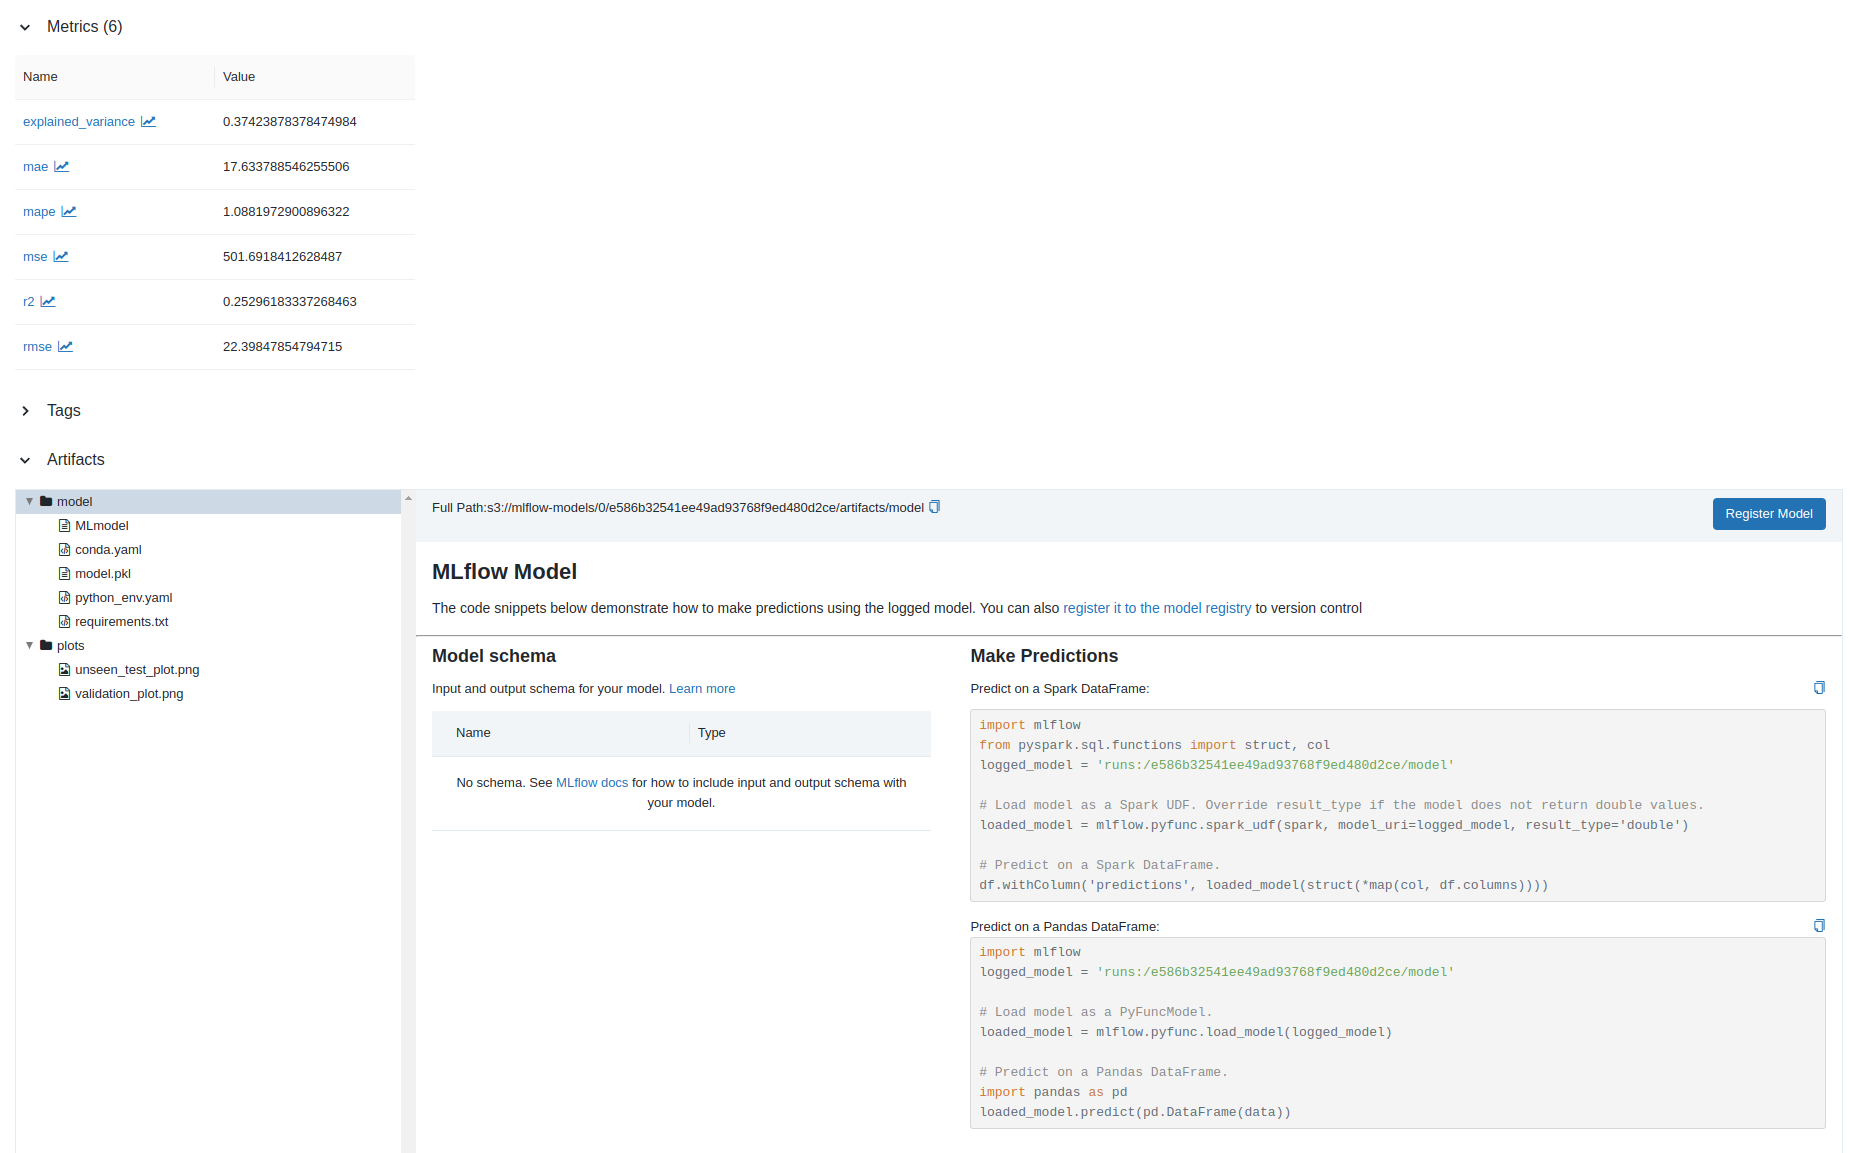
\includegraphics[width=0.93\textwidth]{figures/Mlflow_model_metrics.png}
    \caption{MlFlow Metrics Tracking}
    \label{fig:mlflow_metrics}
\end{figure}

Overall the model tuning process already presents a robust foundation for exploring hyperparameters, but to further enhance this exploration, integrating diverse LSTM architectures could provide a significant leap in model sophistication. This approach not only would broaden the experimental scope but also aligns with the initial strategy of implementing a customizable LSTM model, which has proven instrumental in simplifying the documentation and understanding of the model's structure. Further expansion into varied LSTM designs could unveil new insights and performance benchmarks in the models predictive capabilities.

\section{Model Evaluation}
\label{section:model_evaluation}
The models have been evaluated on the unseen test dataset (Section \ref{section:splitting_dataset}), which is made up of 327 time steps.

\subsection{Metrics}
The top two models have been evaluated using the following metrics:
\begin{itemize}
    \item \textbf{Explained variance (EV):} A measure of how well the model explains the variance in the target variable. A higher EV value indicates that the model is able to capture a greater portion of the underlying patterns in the data.
    \item \textbf{Mean absolute error (MAE):} A measure of the average difference between the predicted and actual values of the target variable. The lower the value the more accurate the predictions are. 
    \item \textbf{Mean squared error (MSE):} A measure of the average squared difference between the predicted and actual values of the target variable. A lower MSE value indicates that the model's predictions are closer to the actual values. 
    \item \textbf{Root mean squared error (RMSE):} This metric is the square root of the MSE and provides an indication of the standard deviation of the errors. A lower RMSE value indicates that the model's predictions are more consistent and less spread out. 
    \item \textbf{Mean absolute percentage error (MAPE):} A measure of the average absolute percent error for each prediction compared to the actual values. MAPE expresses the accuracy as a percentage, providing a simple and intuitive understanding of the model's predictive performance. A lower MAPE value indicates that the model's predictions are closer to the actual values in terms of percentage, making it particularly useful for understanding the relative error in cases where the target variable spans a wide range of values.
    \item \textbf{R-squared (\( R^2 \)):} A measure of the proportion of the variance in the target variable that can be attributed to the model. A higher \( R^2 \) value indicates that the model is able to explain a greater portion of the variance in the data, but it does not necessarily mean the model is good in an absolute sense. \\
\end{itemize}

\subsection{Model 1: amusing-wren-58}
This section provides a detailed evaluation of Model 1 \texttt{amusing-wren-58}, demonstrating its predictive performance through key statistical metrics and a visual comparison of predicted versus actual prices.

\begin{table}[H]
\centering
\begin{tabular}{l l p{10cm}}
\textbf{Metric} & \textbf{Value} & \textbf{Explanation} \\
\hline
EV & 0.838 & The EV score of 0.838 suggests that the model accounts for approximately 83.8\% of the variance in the target variable. This indicates a strong ability of the model to capture the underlying trends and patterns in the data. \\
MAE & 10.64 & The MAE value implies that the model's predictions are, on average, 10.64 units from the actual values. While this shows a degree of accuracy, there is potential for the model to be more precise. \\
MSE & 175.89 & The MSE value signifies that the models errors, when squared, average to this value. Although lower would be better, this indicates a moderately accurate model that may benefit from further refinement. \\
RMSE & 13.26 & The RMSE value reflects the model's prediction consistency. It is a measure of dispersion, showing that the model's errors are generally not too spread out, which suggests a reliable model performance. \\
MAPE & 0.6574 & With a MAPE of 65.74\%, this metric reveals that the model's predictions deviate from the actual values by this percentage on average. This relatively high value points to an area where the model could be improved for better accuracy. \\
\( R^2 \) & 0.821 & The coefficient of determination, or \( R^2 \), is 0.821, indicating that the model effectively captures 82.1\% of the variability in the data. This underscores a strong predictive capability, but it does not necessarily mean the model is good. \\
\end{tabular}
\caption{Model 1 - Metrics and Evaluation (amusing-wren-58)}
\label{table:model_1_evaluation}
\end{table}

The displayed plot (Figure \ref{fig:amusing-wren})  features two lines, where the blue line indicates the actual closing prices, and the orange line represents the predictions made by Model 1: amusing-wren-58. Upon examination, the model's predictions roughly track the actual prices for the most part, reflecting a decent  understanding of the price movement patterns. Both lines exhibit similar trends and volatilities, indicating that the model has a grasp of the temporal dynamics of the price data. \\

\begin{figure}[H]
    \centering
    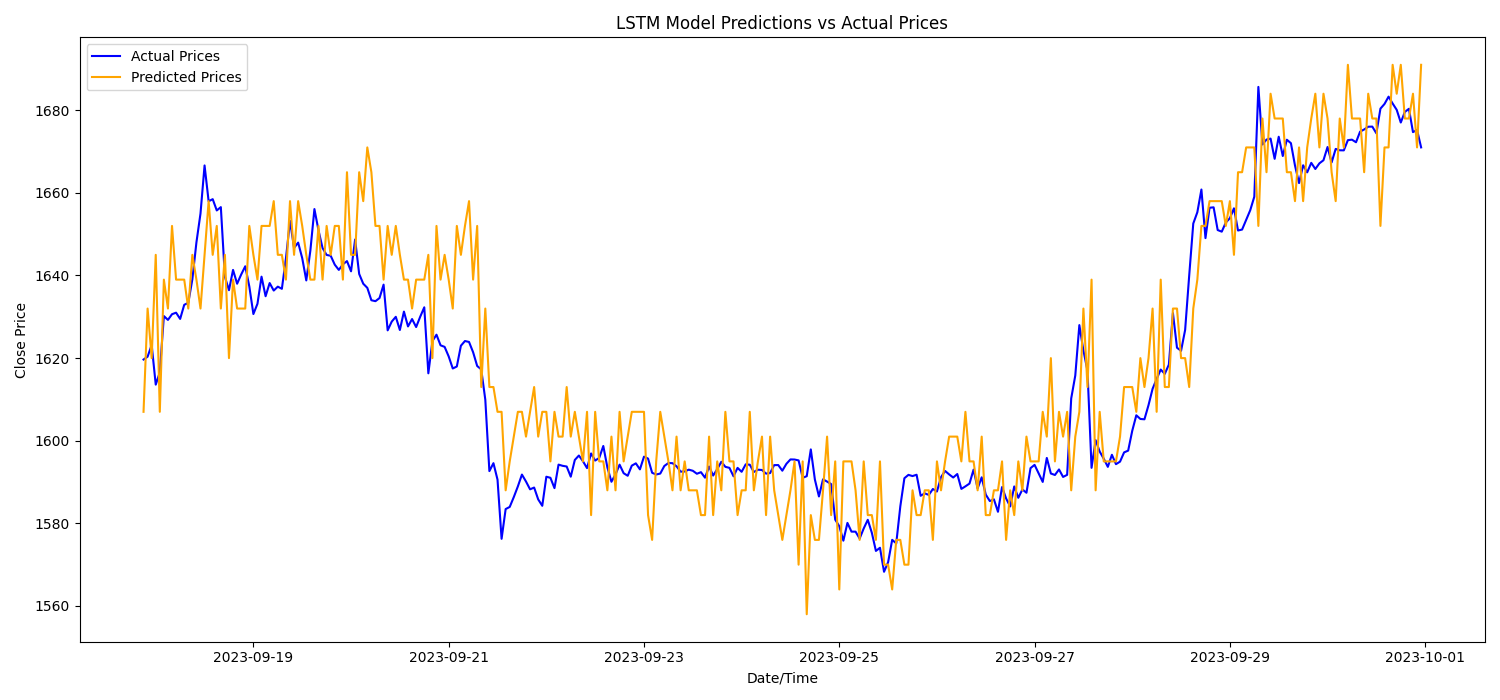
\includegraphics[width=\textwidth]{figures/amusing-wren-58.png}
    \caption{Model 1 - Prediction vs Actual Prices (amusing-wren-58)}
    \label{fig:amusing-wren}
\end{figure}

However, there are noticeable instances where the predicted prices do not align with the actual prices, such as during periods of sideways moving markets, for example in the time period between 2023-09-21 and 2023-09-25, but it does seem to catch rapid peaks quite well between 2023-09-27 and 2023-09-29. These discrepancies might be attributed to the model's limitations in capturing sudden market shifts or anomalies. Despite this, the overall alignment of the two lines throughout the plot signals a decent predictive performance, corroborated by the model's high explained variance score and the tight clustering indicated by the mean absolute error and root mean squared error metrics. The R-squared value of 0.821 further substantiates the model's ability to accurately reflect the majority of the variability in the closing prices, but there is definitely the need for refinement as the model seems to be very sensitive and easily swings far beyond the true values during relatively stable periods. 
\clearpage
\subsection{Model 2: clean-mare-368}
The model 2 \texttt{clean-mare-368} achieved the following scores: 

\begin{table}[H]
\centering
\begin{tabular}{l l p{10cm}}
\textbf{Metric} & \textbf{Value} & \textbf{Explanation} \\
\hline
EV & 0.897 & The EV of 0.897 suggests that the model explains approximately 89.7\% of the variance in the target variable, which indicates the model is capturing most of the variability in the data. \\
MAE & 8.74 & The MAE value suggests that, on average, the model's predictions are approximately 8.74 units away from the actual price. Given the scale of the price, this seems to be a reasonably low error, indicating the model's predictions are fairly accurate. \\
MSE & 121.07 & The MSE value is a measure that squares the errors, penalizing larger errors more severely. This value being relatively low is indicative of the model not making a lot of large errors when inferring the close price. \\
RMSE & 11.00 & The RMSE value indicates that the model's predictions are consistent and less spread out, emphasizing its improved accuracy and reliability compared to Model 1. \\
MAPE & 0.540 &  A MAPE of 0.540, or 54.0\%, is still relatively high even though the other metrics have improved compared to Model 1. This might indicate that while the model performs well in general, it may have periods where its predictions are off by a larger percentage, which could pose a weak point. \\
\( R^2 \) & 0.877 & The \( R^2 \) value is strong, indicating that the model does a good job of fitting the data and can explain a large proportion of the variance. \\
\end{tabular}
\caption{Model 2 - Metrics and Evaluation for Cryptocurrency Price Prediction}
\label{table:new_model_evaluation}
\end{table}

From the graph (Figure: \ref{fig:clean-mare}) and the metrics (Table: \ref{table:new_model_evaluation}) provided, it can be infered that the model's strength lies in its ability to capture the general trend of the actual closing prices, as indicated by the high EV and R-squared values. It also makes predictions that are, on average, quite close to the actual values (low MAE and RMSE). However, the graph shows that at certain points, particularly around the peaks and troughs, the model predictions diverge from the actual prices. This could be due to the model not capturing some of the more volatile movements in the price data, which could be considered a weak point. The high MAPE value suggests that there are instances where the percentage error is quite large, which might occur during these volatile periods, indicating a potential area for improvement in model performance. 

\begin{figure}[H]
    \centering
    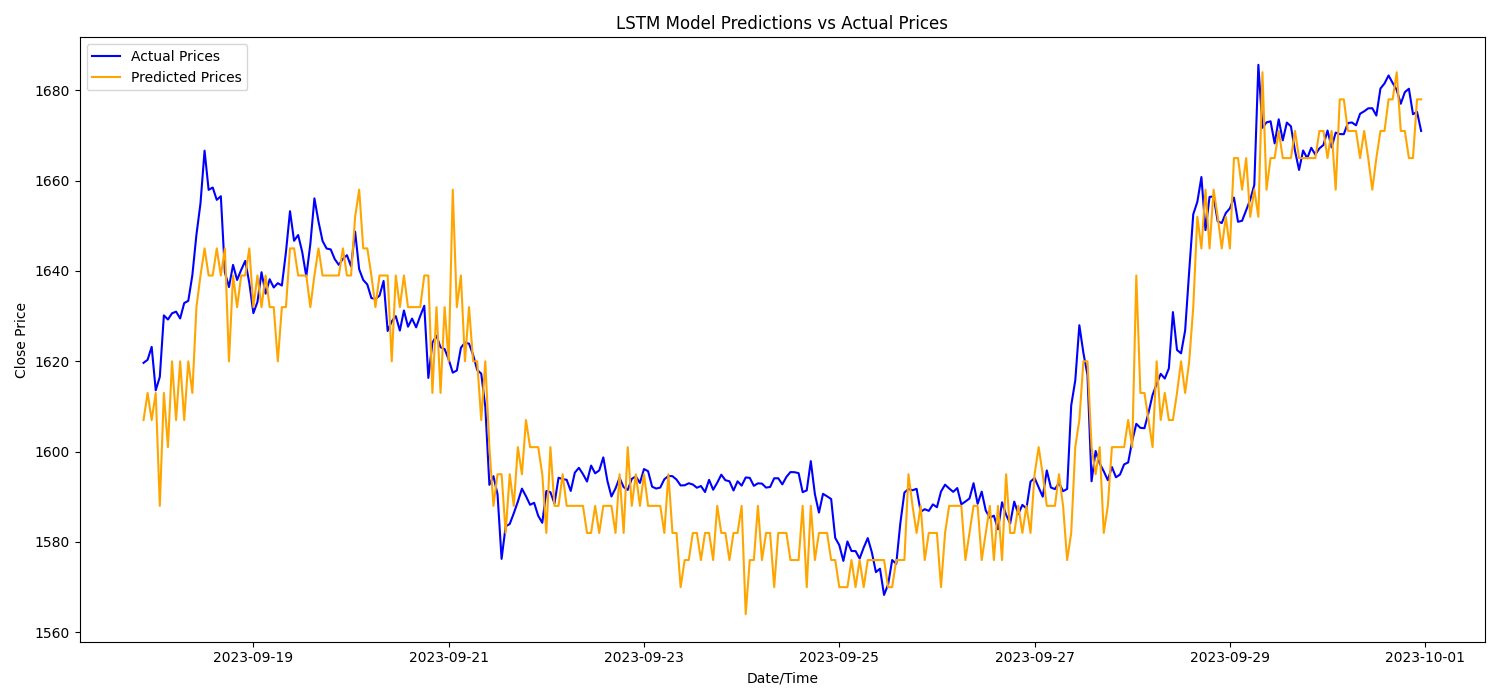
\includegraphics[width=\textwidth]{figures/clean-mare-368.png}
    \caption{Model 2 - Prediction vs Actual Prices (clean-mare-368)}
    \label{fig:clean-mare}
\end{figure}

\subsection{Model Architecture Comparison}
In the following section, the key architectural differences between Model 1 and Model 2 are outlined, which may account for the improved performance in Model 2.

\subsubsection{LSTM Structure}
For Model 1, shown in Listing \ref{lst:model_1_architecture}, the architecture comprises of three LSTM layers, with 228 units each. The first two LSTM layers have the \texttt{return\_sequences} parameter set to True, indicating that they return the full sequence to the next layer. This setup is typical in stacked LSTM configurations where the sequence information should be maintained. The third LSTM layer has \texttt{return\_sequences} set to False, which means it only returns the final output, preparing the data to be fed into the Dense layer. The Dense layer serves as the output layer with a single unit and uses the \texttt{selu} activation function, which is a scaled exponential linear unit that can lead to better convergence during training and seemed to improve the model performance compared to other activation functions (e.g., relu).

\begin{lstlisting}[language=python, caption={Model 1 Structure (amusing-wren-58)}, label={lst:model_1_architecture}]
[{'type':'LSTM', 'units':228, 'return_sequences':True, 'input_shape':(12, 19)},
{'type':'LSTM', 'units':228, 'return_sequences':True},
{'type':'LSTM', 'units':228, 'return_sequences':False},
{'type':'Dense', 'units':1, 'activation':'selu'}]
\end{lstlisting}

Model 2 (Listing \ref{lst:model_2_architecture}) follows a very similar structure but with each LSTM layer containing 240 units, slightly more than Model 1. Additionally, the input shape reflects one additional feature in the data (20 features instead of 19), which could potentially capture more information about the system being modeled. The increased number of units in the LSTM layers may allow Model 2 to learn more complex patterns or relationships in the data, which could be a reason for its improved performance.

\begin{lstlisting}[language=python, caption={Model 2 Structure (clean-mare-368)}, label={lst:model_2_architecture}]
[{'type': 'LSTM', 'units': 240, 'return_sequences': True, 'input_shape': (12, 20)}, 
{'type': 'LSTM', 'units': 240, 'return_sequences': True}, 
{'type': 'LSTM', 'units': 240, 'return_sequences': False}, 
{'type': 'Dense', 'units': 1, 'activation': 'selu'}]
\end{lstlisting}

Both models conclude with a Dense output layer with the same \texttt{selu} activation function, suggesting that the key architectural differences lie in the number of units in the LSTM layers and the dimensionality of the input data.

\subsubsection{Parameters}

The parameters for Model 1 and Model 2 are very similar and both models have been trained on the same dataset. For clarity, the dataset preparation is detailed in Section \ref{section:data_preparation}.

\begin{table}[h!]
\centering
\begin{tabular}{|l|l|}
\hline
\textbf{Parameter} & \textbf{Value} \\
\hline
Learning Rate & 0.001 \\
\hline
Lookback Period & 12 \\
\hline
Metrics & mean\_absolute\_error, mean\_squared\_error, accuracy \\
\hline
Full Dataset Size & 32361 \\
\hline
Training Data Size & 25879 \\
\hline
Validation Set Size & 6470 \\
\hline
Unseen Test Data Size & 327 \\
\hline
Optimizer & Adam \\
\hline
Data Type & numpy.float32 \\
\hline
Batch Size & 16 \\
\hline
\end{tabular}
\caption{Shared Parameters for Model 1 and Model 2}
\label{table:shared_parameters}
\end{table}

The primary difference in parameters between the two models is the set of features used as input data, which are as follows:

\begin{itemize}
    \item Model 1 Features: \{'is\_holiday', 'close\_price', 'volume', 'is\_weekend', 'count', 'hour\_cos', 'hour\_sin', 'day\_of\_week\_cos', 'day\_of\_week\_sin', 'month\_cos', 'month\_sin', 'day\_of\_month\_sin', 'day\_of\_month\_cos', 'year\_normalized', 'close\_lag12', 'close\_lag96', 'ema\_12\_close\_price', 'ema\_48\_close\_price', 'ema\_96\_close\_price'\}
    \item Model 2 Features: \{'is\_holiday', 'close\_price', 'volume', 'is\_weekend', 'count', 'hour\_cos', 'hour\_sin', 'day\_of\_week\_cos', 'day\_of\_week\_sin', 'month\_cos', 'month\_sin', 'day\_of\_month\_sin', 'day\_of\_month\_cos', 'year\_normalized', 'close\_lag12', 'close\_lag96', 'ema\_12\_close\_price', 'ema\_48\_close\_price', 'ema\_96\_close\_price', 'ema\_168\_close\_price'\}
\end{itemize}

The additional feature \texttt{ema\_168\_close\_price} in Model 2 could be a contributing factor to its improved performance. One of the key differences is the loss function used during training. Model 2 uses Mean absolute percentage error as the loss function, which directly optimizes percentage errors, possibly leading to improved performance in metrics that are based on percentages, such as MAPE itself. Model 1 has been trained using the Mean absolute error, which optimizes for absolute differences without considering the relative scale of the target variable, potentially making it less sensitive to proportionally large errors that could be more impactful in a financial context. \\

These differences suggest that Model 2 may be better at capturing both the short- and long-term dependencies in the data due to the additional feature and increased complexity of the LSTM layers and the more ideal loss function.

\subsection{Model Performance Comparison and Conclusion}
Comparing the performance of Model 1: amusing-wren-58 and Model 2: clean-mare-368, several insights can be drawn from their respective metrics and visual analysis. Model 2 demonstrates a notable improvement over Model 1 across several key metrics, highlighting its enhanced predictive capabilities. \\

Model 2's Explained Variance (EV) of 0.897 significantly surpasses Model 1's EV of 0.838, indicating a superior ability to capture the variance in the target variable. This higher EV suggests that Model 2 is more adept at understanding the underlying patterns and trends in the data. \\

The Mean Absolute Error (MAE) further cements Model 2's lead with a value of 8.74, compared to Model 1's MAE of 10.64. This reduction in MAE signifies that Model 2's predictions are closer to the actual values, showcasing its heightened accuracy. \\

In terms of the Mean Squared Error (MSE) and Root Mean Squared Error (RMSE), Model 2 again outperforms Model 1 with lower values of 121.07 and 11.00, respectively. These metrics indicate that Model 2 not only makes fewer large errors but also maintains a consistent level of prediction accuracy across the dataset. \\

However, the Mean Absolute Percentage Error (MAPE) reveals a nuanced perspective. Although the 54.0\% MAPE for Model 2 might appear elevated at first glance, it is essential to not lean on this figure alone and consider all metrics. It does indicate that Model 2 generally delivers reasonable results, yet it encounters challenges in accurately predicting certain cases or outliers, leading to significant discrepancies from the true values. \\

The R-squared value for Model 2 stands at 0.877, an improvement over Model 1's 0.821. This indicates that Model 2 is better at modeling the variance in the data, providing a more accurate representation of the market dynamics. \\

In conclusion, Model 2: clean-mare-368 shows a clear advancement in predictive performance over Model 1: amusing-wren-58, evidenced by its superior metrics across the board. Model 2 demonstrates its enhanced ability to accurately capture and predict the underlying trends within the dataset. While the MAPE suggests room for improvement in handling outliers or specific market conditions, the overall metrics indicate a robust model capable of providing valuable insights. These findings underscore the importance of comprehensive model evaluation, beyond a single metric, to truly understand and appreciate a model's predictive power and potential limitations.
 

\section{Backend}
As the backbone of any robust machine learning system, the backend architecture requires careful consideration of performance, stability, and security. Rust, an emerging systems programming language, offers a compelling combination of features making it an excellent choice for the backend.

\subsection{Rust Libraries for Backend Services}

To build a backend that is both performant and scalable, a suite of Rust libraries have been utilized, each serving a distinct purpose in the backend architecture. The following libraries form the core of the backend:

\begin{itemize}
    \item \textbf{Axum \cite{AxumDocumentation}} Version 0.7.2 of the Axum library is used for crafting web applications. Axum leverages the asynchronous runtime of Tokio and focuses on ergonomics and modularity. 
    \item \textbf{Tokio \cite{TokioDocumentation}} The asynchronous runtime Tokio, version 1.23, provides a non-blocking event loop that drives the application's I/O operations.
    \item \textbf{Serde \cite{SerdeDocumentation}} Serialization and deserialization within the service are handled by Serde, version 1.0, a framework enabling efficient, declarative, and generic data serialization. The "derive" feature is activated, allowing for the automatic generation of code to serialize and deserialize custom data structures.
    \item \textbf{Sqlx \cite{SQLxDocumentation}} The Sqlx library, version 0.7.3, is chosen for database interactions. It provides compile-time checked queries and supports various databases, including PostgreSQL.
\end{itemize}

These libraries form a modern tech stack that bolsters the backend's capacity to handle web services, asynchronous processing, data serialization, and database management efficiently and securely.

\subsection{Collector Module}
\label{section:collector}

The \textbf{Collector Module} serves as the data acquisition gateway of the system. It is implemented to connect with real-time data feeds and extract valuable trade information, thereby feeding the system's analytics and decision-making processes.

\subsubsection{Kraken WebSockets API Overview}
The Kraken WebSockets API \cite{KrakenWebsocketsDocumentation} provides a real-time streaming service for cryptocurrency market data. Through WebSocket connections, clients can subscribe to various data channels to receive immediate updates, a feature that the system takes full advantage of for collecting trade data.

\paragraph{Efficient Data Streaming}
The efficient streaming of live data via the Kraken WebSockets API is instrumental for applications that depend on up-to-the-minute market information, such as algorithmic trading platforms and analytical tools. By leveraging this API, the backend system, is able to collect, process, and utilize market data in a way that aligns with the high-throughput and low-latency requirements of modern trading systems.

\paragraph{Trade Subscription}
Subscribing to trade data is a key feature of the API. The trade subscription (Listing \ref{lst:trade_sub}) provides a live feed of trade executions on the exchange, including details such as price, volume, and time. The payload structure for trade messages (Listing \ref{lst:trade_payload}) consists of multiple fields (price, volume, time, side, order type, misc), ensuring that clients have access to comprehensive trade data for their selected currency pairs.


\begin{lstlisting}[language=bash, caption={Subscription for Trade Data}, label={lst:trade_sub}]
{
  "event": "subscribe",
  "pair": [
    "XBT/USD"
  ],
  "subscription": {
    "name": "trade"
  }
}
\end{lstlisting}

\begin{lstlisting}[language=bash, caption={Trade Message Payload}, label={lst:trade_payload}]
[
  0,
  [
    [
      "5541.20000",
      "0.15850568",
      "1534614057.321597",
      "s",
      "l",
      ""
    ],
    [
      "6060.00000",
      "0.02455000",
      "1534614057.324998",
      "b",
      "l",
      ""
    ]
  ],
  "trade",
  "XBT/USD"
]
\end{lstlisting}

\subsubsection{Functionality and Workflow}
The collector initiates a WebSocket connection to the Kraken exchange, subscribing to trade data (Listing \ref{lst:trade_sub}) streams for various cryptocurrency pairs. It maintains a mapping of currency symbols to their corresponding database identifiers, ensuring that incoming trade data can be accurately categorized and stored. \\

Upon receiving a new trade message, the collector performs several critical operations:
\begin{itemize}
    \item Parses the message and filters out non-trade related information such as heartbeats and subscription acknowledgments.
    \item Inserts new trading symbols into the database if they do not exist already, expanding the system's ability to track a broader range of currency pairs.
    \item Converts trade data into internal models and persists them into the database using the trade repository's insertion functionality.
\end{itemize}

The collector's loop continues to listen for new subscription messages and trade data, maintaining an up-to-date and comprehensive dataset for the system.

\paragraph{Asynchronous and Parallel Processing}
The collector is built to leverage Rust's asynchronous runtime and parallel processing capabilities, allowing it to handle high volumes of data with minimal latency. It uses the \texttt{tokio} and \texttt{rayon} libraries to perform non-blocking data operations and parallel computations.

\paragraph{Error Handling and Logging}
Robust error handling is embedded within the collector, ensuring that any issues encountered during data collection or insertion are logged and managed appropriately. This proactive approach to monitoring ensures the system's reliability and data integrity.

In essence, the trade data collector serves as a resilient and efficient backend module, tasked with the continuous collection of trade data, which forms the backbone of the system's data-driven analytics and machine learning capabilities.

\subsection{Webserver}
The backend webserver exhibits a modular design that significantly enhances the system's flexibility and maintainability. This is achieved by splitting the applications into distinct components, where each component is responsible for a specific aspect of the system's functionality.

\begin{itemize}
\item \textbf{Server Module}: Acts as the entry point of the application, handling server initialization and configuration (Listing \ref{lst:webserver_main}).
\begin{lstlisting}[language=rust, caption={Webserver Main}, label=lst:webserver_main]
#[tokio::main(flavor = "multi_thread", worker_threads = 6)]
async fn main() -> Result<(), ()> {
    dotenv().ok();
    logger::run().await;
    info!("server is starting up ...");

    let (sender, receiver) = mpsc::channel(1);

    collector::collector::run(receiver).await;
    webserver::webserver::run(sender).await;
    Ok(())
}
\end{lstlisting}

\item The \textbf{Webserver Module} is architected to set up the web routing and middleware configurations that dictate the processing of HTTP requests and generation of responses. This module uses the Axum framework, renowned for its ergonomic design and powerful features, to define clear and concise routes for different endpoints. Each route is associated with a specific handler function that executes when the route is accessed.

Middleware components are strategically placed to manage cross-cutting concerns that apply across multiple routes. These concerns include but are not limited to logging for monitoring and debugging, authentication to secure endpoints, and error handling to gracefully manage any unexpected conditions during request processing.

The module is designed with modularity at its core, with routes organized into distinct sub-modules, which enhances the clarity and scalability of the codebase, allowing for independent development and testing of different API endpoints. A CORS layer has been incorporated to ensure that the server can interact with web clients from different origins, making it versatile and web-friendly.

Below is the setup code for the Axum webserver, detailing the initialization process, and the middleware and routes configuration:

\begin{lstlisting}[language=rust, caption={Webserver Axum Setup with Annotations}, label=lst:axum_webserver_init]
pub async fn run(sender: tokio::sync::mpsc::Sender<String>) {
    // Initialize database connection and application state.
    let pool = postgresdb::get_connection().await; 
    let app_state = AppState::new(pool.clone(), /* Redis cache */ None, sender);

    // Configure CORS to allow interactions from any origin.
    let cors = CorsLayer::new()
        .allow_methods(Any)
        .allow_origin(Any)
        .allow_headers(Any);

    // Define the router and its associated routes.
    let app = Router::new()
        .route("/ping", get(ping))
        .merge(routes::ohlc::routes::router(pool).await) 
        .merge(routes::symbol::routes::router(app_state).await) 
        .merge(routes::import::routes::router(pool).await) 
        .merge(routes::modelexecution::routes::router(pool).await) 
        .merge(routes::trade::routes::router(pool).await) 
        .merge(routes::upload::routes::router().await) 
        .layer(cors); // Apply CORS settings to all routes

    // Determine server address and start listening for requests.
    let address = SocketAddr::from(get_address().await);
    let listener = TcpListener::bind(address).await.unwrap();
    axum::serve(listener, app.into_make_service())
        .await
        .unwrap_or_else(|_| panic!("Server cannot launch."));
}
\end{lstlisting}

\item The \textbf{Service Module} within the system architecture encapsulates specialized sub-modules, each dedicated to a distinct set of data management and operational tasks:

\begin{itemize}
    \item \textbf{Import Sub-Module}: Oversees the importation process of historical data, ensuring the database can be populated with historical datasets and materialized views are refreshed to account for the newly imported data.
    \item \textbf{Symbol Sub-Module}: Manages the retrieval and management of symbol data, interfacing directly with the \texttt{symbol\_repository} to ensure up-to-date symbol information is available.
    \item \textbf{Trade Sub-Module}: Handles the acquisition of live trade data, utilizing the \texttt{trade\_repository} to fetch and process trade transactions from the market.
    \item \textbf{OHLC Sub-Module}: Deals with the retrieval of Open-High-Low-Close (OHLC) data, critical for market analysis, by making use of the \texttt{ohlc\_repository}.
    \item \textbf{Model Execution Sub-Module}: Orchestrates the execution of machine learning models, coordinating the loading of model configurations and relevant data from Timescale. It facilitates model execution requests to the model service, which ultimately yield predictive outcomes such as the estimated close\_price.
\end{itemize}

Each submodule within the service module is linked to a specific domain, ensuring the separation of concerns and efficient data handling that is crucial for the system's responsiveness and analytical capabilities. \\

The following code snippet showcases an example of the \texttt{symbol\_service}. This service is responsible for retrieving symbol data from the repository and transforming it into a data transfer object (DTO) format that is optimized for client-side consumption.

\begin{lstlisting}[language=rust, caption={Symbol Service Fetch Function}, label=lst:symbol_service]
pub async fn get_symbols(pool: &sqlx::PgPool) -> Result<Vec<SymbolDto>, GenericError> {
    match symbol_repository::get_symbols(pool).await {
        Ok(data) => {
            let result: Vec<SymbolDto> = data
                .into_par_iter()
                .map(|model| SymbolDto::from(&model))
                .collect();

            Ok(result)
        }
        Err(err) => {
            Err(err)
        },
    }
}
\end{lstlisting}

This function demonstrates a typical service operation, where data is fetched from the repository and transformed. The use of parallel iteration through \texttt{into\_par\_iter} signifies the system's commitment to performance and efficiency.

\item \textbf{Repository Module}: Encapsulates all database interactions, abstracting the complexity of data queries and manipulations. It is further divided into sub-modules for different domain entities like symbols (Listing \ref{lst:symbol_repository}), trades, and OHLC data, promoting a single responsibility principle.
\begin{lstlisting}[language=rust, caption={Symbol Repository Example}, label=lst:symbol_repository]
const QUERY_SELECT_SYMBOLS: &str = "SELECT * FROM symbol;";

pub async fn get_symbols(
    pool: &sqlx::PgPool,
) -> Result<Vec<SymbolModel>, GenericError> {
  match sqlx::query(QUERY_SELECT_SYMBOLS)
      .map(|row: PgRow| SymbolModel::from(row))
      .fetch_all(pool)
      .await
  {
      Ok(data) => Ok(data),
      Err(err) => Err(RepositoryError::general_error(err.to_string())),
  }
}
\end{lstlisting}

\item The \textbf{Utils Module} offers a suite of utility functions and shared libraries that facilitate cross-application use, significantly increasing code reusability. For instance, Listing \ref{lst:webserver_address_util} showcases a utility function that retrieves the address configuration for the webserver. While this function is currently tailored for the webserver, it can be refactored to generically obtain host IP addresses and ports for various services by reading from the environment configuration. Such a modification would enhance the module's reusability across different components of the application.
\begin{lstlisting}[language=rust, caption={Util get\_address for Webserver}, label=lst:webserver_address_util]
pub async fn get_address() -> (IpAddr, u16) {
    let host_ip_address =
        std::env::var("WEBSERVER_IP").unwrap_or_else(|_| panic!("WEBSERVER_IP must be set!"));
    let host_port =
        std::env::var("WEBSERVER_PORT").unwrap_or_else(|_| panic!("WEBSERVER_PORT must be set!"));

    let ip_address = host_ip_address
        .parse::<IpAddr>()
        .expect("IP Adress invalid");
    let port = host_port.parse::<u16>().expect("PORT is invalid.");

    let url_message = format!(
        "executed: initializing server url = {}:{}",
        &ip_address, &port
    );
    info!(url_message);

    (ip_address, port)
}
\end{lstlisting}


\end{itemize}

\paragraph{Separation of Concerns}
This modular setup is grounded in the separation of concerns principle, which dictates that each module should address a separate piece of the application's functionality. By adhering to this principle, the application not only becomes more manageable and easier to understand but also enhances each module's reusability and testability. \\

The modular nature of this setup makes the webserver highly flexible, allowing for the addition or modification of routes and middleware without disrupting existing functionality. It embodies a cleanly separated architecture that simplifies concern isolation, ultimately leading to a system that is easier to extend, maintain, and troubleshoot.

\subsubsection{Error Handling}
A robust error handling system is vital for maintaining the reliability and predictability of any application. In the provided setup, the system uses a combination of a trait, a struct, and an enumeration to structure and manage errors effectively.

\paragraph{GenericErrorTrait}
The \texttt{GenericErrorTrait} (Listing \ref{lst:generic_error_trait}) is a Rust trait that defines a common interface for error handling. Traits in Rust are similar to interfaces in other languages, providing a way to define shared behavior. This trait includes two methods:
\begin{itemize}
    \item \texttt{get\_message()}: Returns a human-readable error message.
    \item \texttt{get\_code()}: Provides a specific error code, useful for categorizing and responding to different error types.
\end{itemize}

\begin{lstlisting}[language=rust, caption={GenericErrorTrait Utils Module}, label=lst:generic_error_trait]
pub trait GenericErrorTrait {
    fn get_message(&self) -> String;
    fn get_code(&self) -> String;
}
\end{lstlisting}

\paragraph{ErrorBody Struct}
The \texttt{ErrorBody} struct (Listing \ref{lst:error_body}) is a concrete representation of an error, containing a message and a code. It implements the \texttt{GenericErrorTrait}, thereby adhering to the interface defined by the trait. 
\begin{lstlisting}[language=rust, caption={ErrorBody Utils Module}, label=lst:error_body]
#[derive(Debug)]
pub struct ErrorBody {
    message: String,
    code: String,
}
\end{lstlisting}

\paragraph{GenericError Enum}
The \texttt{GenericError} (Listing \ref{lst:generic_error}) enumeration is a versatile way to encapsulate different error types while maintaining a uniform interface. It has variants for different error contexts, such as \texttt{Repository}, \texttt{Service}, and \texttt{Web}. Each variant holds an \texttt{ErrorBody}, ensuring that every error within the system has a consistent structure.

\begin{lstlisting}[language=rust, caption={GenericError Utils Module}, label={lst:generic_error}]
#[derive(Debug)]
pub enum GenericError {
    Repository(ErrorBody),
    Service(ErrorBody),
    Web(ErrorBody),
}
\end{lstlisting}
\mbox{}\\
This setup offers several advantages:
\begin{itemize}
    \item \textbf{Consistency}: By using a common trait and struct, the system ensures that all errors, regardless of where they occur, have a consistent representation.
    \item \textbf{Flexibility}: The \texttt{GenericError} enum can be easily extended to include more error types as the system evolves.
    \item \textbf{Ease of Use}: The trait and struct provide straightforward methods for creating and handling errors, making the code more readable and maintainable.
    \item \textbf{Error Propagation}: This setup simplifies error propagation across different layers of the application, such as from the repository layer to the web layer.
\end{itemize}

In summary, this error handling system offers a structured and effective approach to managing errors, which is crucial for maintaining the robustness and user-friendliness of the application.

\subsubsection{Environment Configuration}
Employing an environment configuration file is essential for a system that prioritizes security, maintainability, and scalability, ensuring that it remains robust and flexible across various deployment environments. In this case the environment variables have been defined in the docker compose file, which itself makes use of a global \texttt{config.env} file (Section \ref{docker_config_env}) that initializes the environment variables for the backend.


\section{Model Service}

The \textbf{Model Service} operates as a specialized web server within the infrastructure, dedicated to managing the execution of machine learning models. This service plays a pivotal role, closing the gap between the raw data inputs and the derived actionable insights.

\subsection{Operational Workflow}
At its core, the Model Service's primary role involves processing incoming requests that carry both the model configuration (Listing \ref{lst:model_configuration}) and the required data for model inference. Specifically, these requests encompass OHLC (open, high, low, close price) data, volume, and trade count, which are essential for the model inference.

\begin{lstlisting}[language=bash, caption={Model Configuration (JSON)}, label={lst:model_configuration}]
{
  "symbol_id": 1,
  "modelname": "model.pkl",
  "data_type": "np.float32",
  "lookback": 16,
  "lags": [12, 168],
  "window_sizes": [],
  "span_sizes": [6, 12],
  "active": true,
  "features": [
    "is_holiday",
    "close_price",
    "volume",
    "is_weekend",
    "count",
    "hour_cos",
    "hour_sin",
    "day_of_week_cos",
    "day_of_week_sin",
    "month_cos",
    "month_sin",
    "day_of_month_sin",
    "day_of_month_cos",
    "year_normalized",
    "close_lag12",
    "close_lag168",
    "ema_6_close_price",
    "ema_12_close_price"
  ]
}
\end{lstlisting}

The service operates using a singular endpoint, \texttt{/execute}, designed to handle POST requests (Listing \ref{lst:model_service_entry}). Upon receiving a request, the service unpacks the JSON payload, which encapsulates both the model configuration and the necessary data. This configuration delineates all necessary details for the model execution, encompassing the model's name, the input features, parameters, and the comprehensive dataset required for the process. \\

\begin{lstlisting}[language=Python, caption={Model Service Flask Entry Point}, label={lst:model_service_entry}]
from flask import Flask, request, jsonify
from model_execution import * 

app = Flask(__name__)

@app.route('/execute', methods=['POST'])
def execute_model():
    try:
        config = request.json
        model_execution = ModelExecution(config)
        timestamp, price = model_execution.execute()
        return jsonify({"bucket": timestamp, "close_price": price.item()}), 200
    except Exception as e:
        return jsonify({"error": str(e)}), 500

if __name__ == '__main__':
    app.run(debug=False, host='0.0.0.0', port=7000, load_dotenv=True)
\end{lstlisting}

\subsubsection{Model Execution Class}
The initialization of the \texttt{ModelExecution} class (Listing \ref{lst:model_execution_class}) triggers the loading of environment variables via \texttt{load\_dotenv}. These variables play a crucial role in initializing the \texttt{ModelProvider} class. This class bears the responsibility of fetching the machine learning model from an S3-compatible storage solution, specifically MinIO in this context. \\

Upon receiving a request, the \texttt{ModelExecution} class is initialized using the model configuration. This class undertakes the task of transforming the dataset (as detailed in Section \ref{section:data_preparation}), ensuring the inclusion of features as specified in the model configuration. Subsequently, it retrieves the actual model from MinIO (as elaborated in Section \ref{section:minio}). After the model inference, the service compiles a JSON response. This response encapsulates the model's prediction, integrating the relevant timestamp, and providing the inferred close prices.

\begin{lstlisting}[language=Python, caption={Model Execution Class}, label={lst:model_execution_class}]
class ModelExecution:
  def __init__(self, config):
    print("Initializing Model Execution")
    load_dotenv()
    self.config = config

    self.model_provider = ModelProvider(os.getenv('S3_BUCKET'),
                                       config['modelname'],
                                       os.getenv('AWS_ACCESS_KEY_ID'),
                                       os.getenv('AWS_SECRET_ACCESS_KEY'),
                                       os.getenv('S3_ENDPOINT_URL'))

    self.data_service = DataService(os.getenv('BACKEND_ENDPOINT'))

  def execute(self):
    print("Starting execution")
        
    df = pd.DataFrame(self.config['data'])
    df.reset_index(inplace=True)

    data_preperation_service = DataPreparation(df, self.config)

    X = data_preperation_service.prediction_sequence
    X_reshaped = X.reshape(1, int(self.config['lookback']), len(self.config['features']))

    self.model_provider.fetch_model(self.config['modelname'])
    with open(self.config['modelname'], 'rb') as file:
        model = cloudpickle.load(file)

    predicted_price_log = model.predict(X_reshaped, verbose=0)
    predicted_price = np.expm1(predicted_price_log)[0, 0]
        
    parsed_date = datetime.strptime(self.config['from_date'], '%Y-%m-%dT%H:%M:%S%z')
    new_date = parsed_date + timedelta(hours=1)
    output_date = new_date.strftime('%Y-%m-%dT%H:%M:%S') + 'Z'
    print(output_date)
        
    return output_date, predicted_price
\end{lstlisting}

Additionally, the \texttt{DataService} comes into play for interfacing with the backend service for any extra data requirements. Although this class was previously utilized, enhancements have been made to streamline the data flow and minimize execution times by transmitting the required data alongside the initial requests.

The \texttt{ModelExecution} class is at the core of the Model Service, steering the complete lifecycle of executing a machine learning model.

\subsubsection{Significance in the System}
The \texttt{Model Service} is the cornerstone of the system, pivotal for harnessing the power of machine learning in forecasting. By meticulously managing the complexities of model retrieval, data processing, and prediction it ensures that the system delivers precise and timely forecasts, a critical capability in dynamic sectors such as the financial markets.

\section{Frontend}

The frontend of the system is engineered using Angular 17 \cite{AngularOverview} and Node.js \cite{NodejsWebsite}. This combination offers a potent platform for crafting dynamic, responsive, and user-friendly web applications.

\subsection{Dashboard Overview}

The dashboard (Figure \ref{fig:frontend_dashboard}) is a crucial component of the frontend, designed to offer users a comprehensive overview of the system's analytics. It is the focal point for data visualization, presenting both historical and predictive data in an intuitive and accessible manner.
\begin{figure}[ht!]
    \centering
    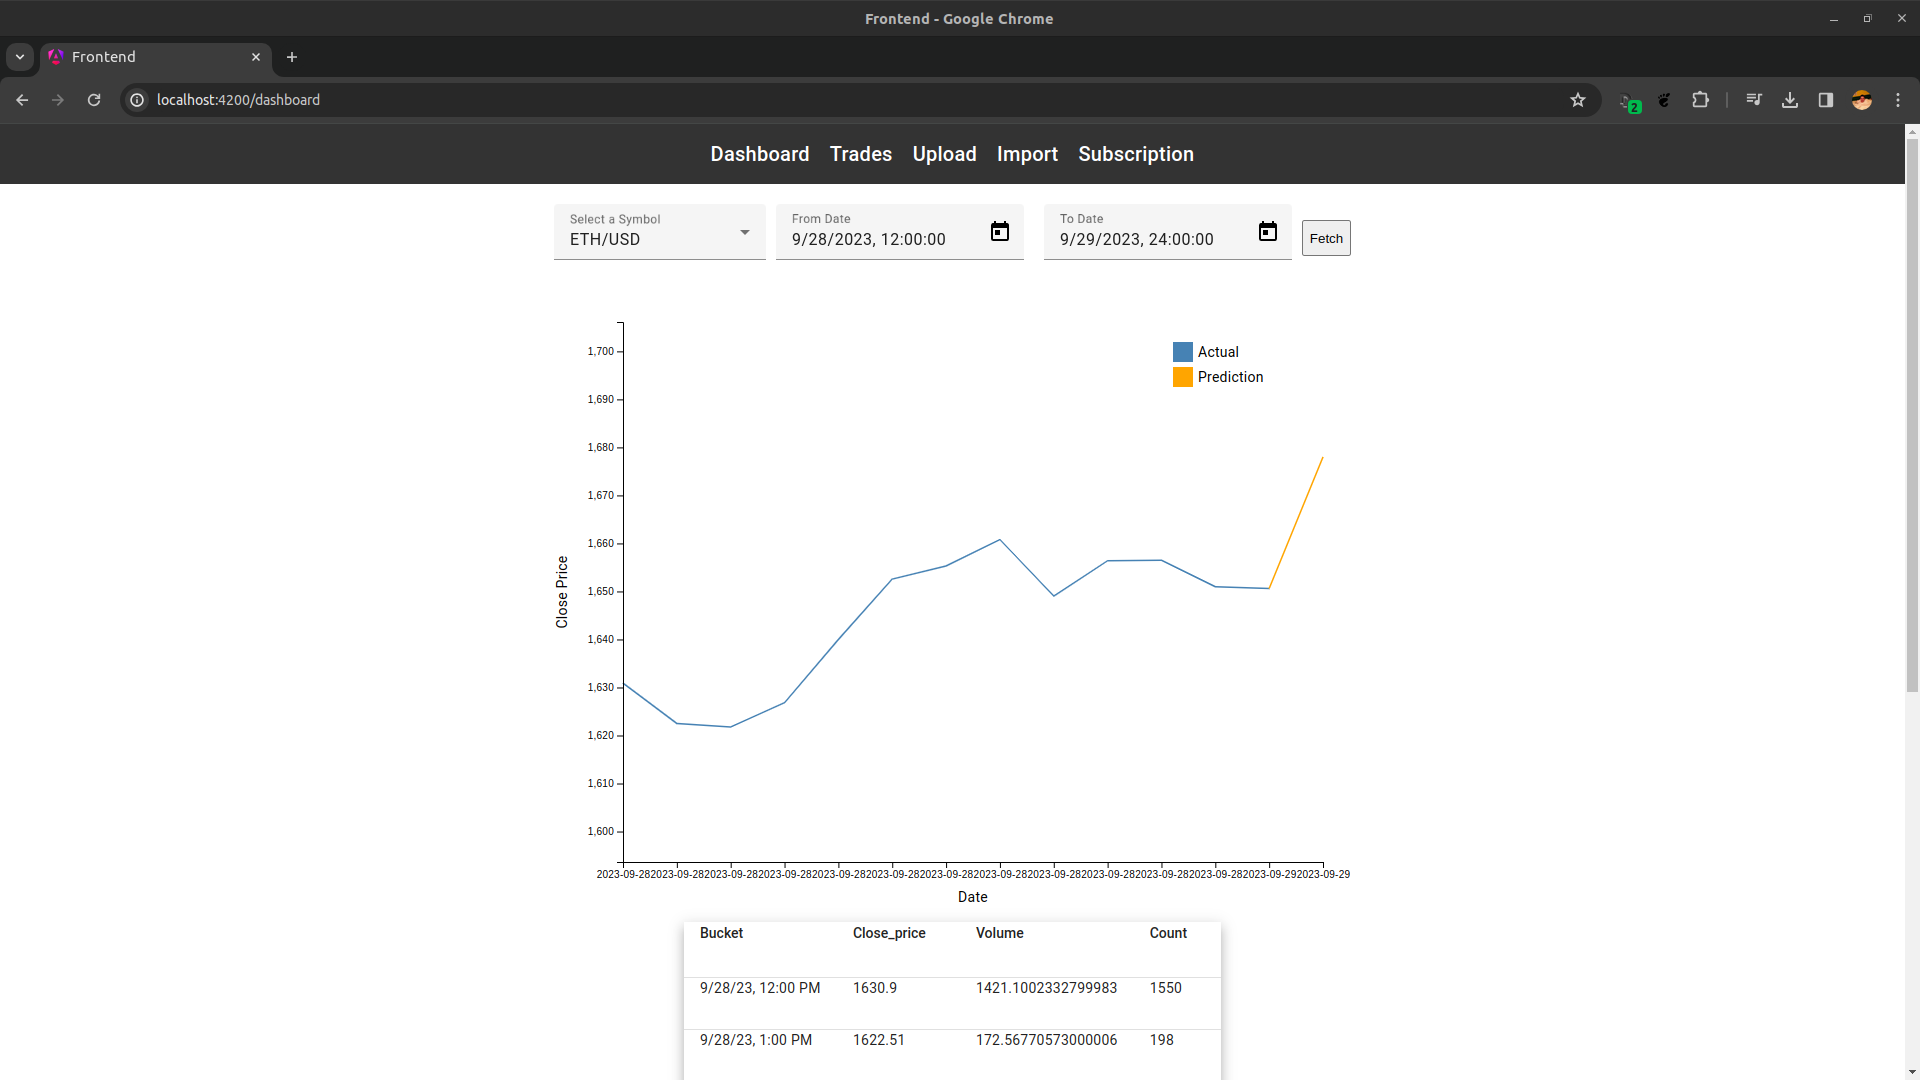
\includegraphics[width=\textwidth]{figures/frontend_dashboard.png}
    \caption{Dashboard}
    \label{fig:frontend_dashboard}
\end{figure}

\subsubsection{User Interface}
The dashboard interface is structured to provide a seamless user experience:
\begin{itemize}
    \item \textbf{Symbol Selection}: Users can choose from a dropdown menu to select different symbols (currency pairs) for which they wish to view a forecast and OHLC data.
    \item \textbf{Date Range}: The dashboard includes a date range picker, allowing users to specify the time frames, they want to analyze.
    \item \textbf{Fetch Data}: The \texttt{Fetch} button initiates the retrieval of data based on the selected symbol and date range, updating the visualizations accordingly.
\end{itemize}

\subsubsection{Data Visualization}
The core of the dashboard is its data visualization:
\begin{itemize}
    \item \textbf{Price Chart}: A line chart prominently displays the close price trends over the selected time period. This chart helps users quickly grasp market movements and identify trends.
    \item \textbf{Prediction Indicator}: Predictive analytics are highlighted on the chart with a distinct color, differentiating predicted values from actual historical data.
\end{itemize}

\subsubsection{Data Table}
Below the chart is a data table that enumerates detailed information:
\begin{itemize}
    \item \textbf{Bucket}: Specific time intervals (e.g., hourly buckets) corresponding to the data points on the chart.
    \item \textbf{Close Price}: Closing price of the asset for each bucket, providing granular insight into price fluctuations.
    \item \textbf{Volume}: Trading volume within each bucket, offering an indication of market activity.
    \item \textbf{Count}: Number of trades that occurred, which can serve as a proxy for market liquidity or activity during the bucket's period.
\end{itemize}


In summary, the frontend dashboard provides a rich, interactive platform for monitoring and analyzing market data. Its intuitive design and visualization make it an essential part of the user interface, enabling effective display and examination of financial data and model predictions.

\subsection{Trades}

The \texttt{Trades} tab (Figure \ref{fig:frontend_trades}) within the frontend is a detailed ledger that presents users with a transaction-level view of trading activity. It complements the aggregate data visualized on the dashboard by providing the granular details of each trade.

\begin{figure}[ht!]
    \centering
    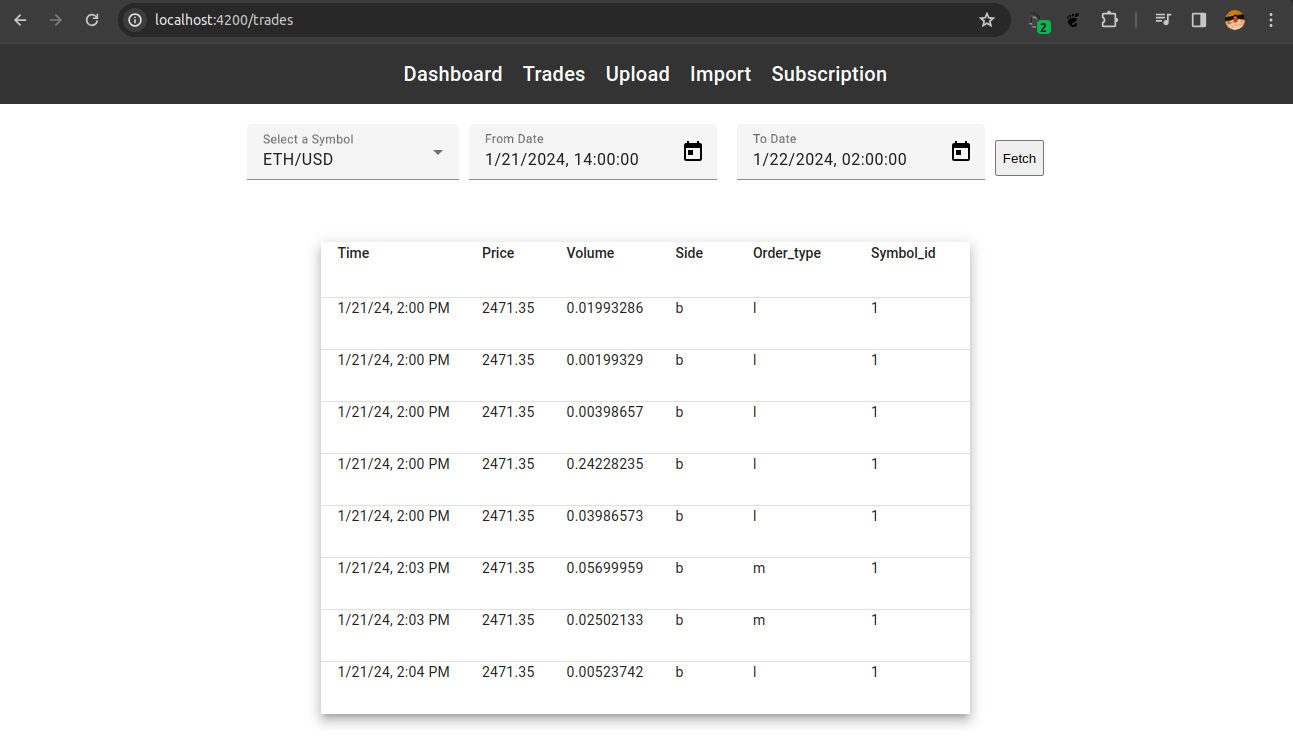
\includegraphics[width=\textwidth]{figures/frontend_trades.png}
    \caption{Trades}
    \label{fig:frontend_trades}
\end{figure}

\subsubsection{Interface and Functionality}
While utilizing the same symbol and date range selectors as the dashboard for consistency and also showcasing the re-usability of angular components, this tab specifically showcases:
\begin{itemize}
    \item A tabular display of trades, listing the time of trade, price, volume, and other details.
    \item Information on the trade side ('b' for buy, 's' for sell) and order type, allows users to discern market behaviors.
    \item The symbol identifier associated with each trade links the data back to the system's internal symbol mapping.
\end{itemize}

The \texttt{Trades} tab serves as an essential tool for users requiring a comprehensive audit of trade history and market dynamics. In essence, this is a vital feature of the frontend, providing an in-depth look at the trade data that drives the analytical engines of the system.

\subsection{Upload Functionality}
\label{section:frontend_upload}

The \texttt{Upload} (Figure \ref{fig:frontend_upload}) tab in the frontend is designed to facilitate the ingestion of historical data into the system via CSV files. This utility is crucial for users who need to input bulk data without manual entry.
\begin{figure}[ht!]
    \centering
    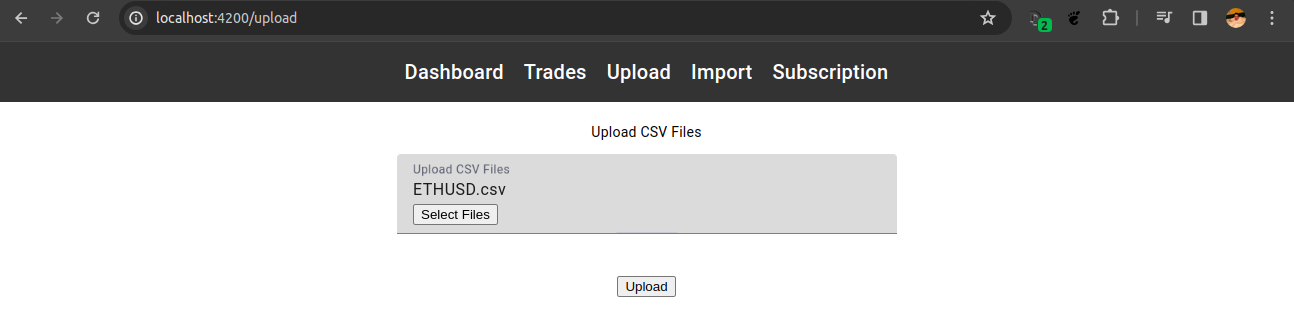
\includegraphics[width=\textwidth]{figures/frontend_upload_file.png}
    \caption{Upload}
    \label{fig:frontend_upload}
\end{figure}

\subsubsection{Interface and Usage}
The interface of the \texttt{Upload} tab is straightforward and user-friendly:
\begin{itemize}
    \item It provides an option to \texttt{Select Files} which opens the user's file explorer to choose the CSV file(s) they intend to upload.
    \item The \texttt{Upload} button is then used to initiate the transfer of the selected file(s) to the system.
\end{itemize}


\subsection{Import Feature}

The \texttt{Import} tab (Figure \ref{fig:frontend_import}) is an essential part of the frontend that enables users to finalize the ingestion of historical data into the system. This feature interfaces with the backend to parse uploaded files and integrate their contents into the database for further processing and analysis.

\begin{figure}[ht!]
    \centering
    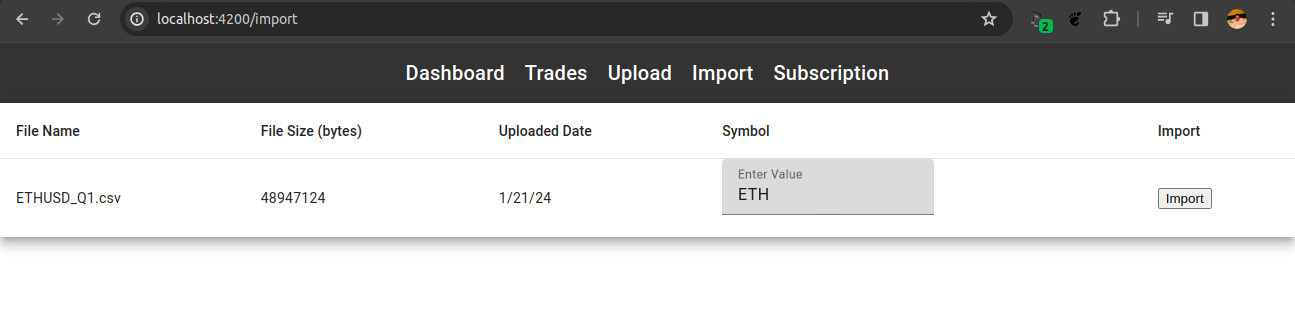
\includegraphics[width=\textwidth]{figures/frontend_import.png}
    \caption{Import}
    \label{fig:frontend_import}
\end{figure}

\subsubsection{Functionality}
The import section provides a streamlined process:
\begin{itemize}
    \item Displays a list of uploaded files, showing essential details like file name, size, and the date of upload.
    \item Allows users to associate each file with a specific symbol. This enables the user to add data from new symbols ensuring that the data is imported using the correct symbol.
    \item The \texttt{Import} button triggers the backend processes to parse the selected file, extract its contents, and import the data into the system's database.
\end{itemize}

\subsubsection{Workflow Integration}
The import functionality acts as a bridge between the initial file upload and the data's operational use within the system. It ensures that the data from the CSV files is properly validated, transformed, and stored, making it available for the system's analytical modules.

\subsubsection{User Empowerment}
This tab empowers users to manage the data lifecycle comprehensively, from uploading raw data files to initiating their integration into the system's core data structures. It is designed to handle large datasets, facilitating efficient data management and scalability.

In summary, the \texttt{Import} tab is a critical feature that encapsulates the system's capability to assimilate external data sources, providing users with control over when and how data is incorporated into the system.

\subsection{Subscription Management}

The \texttt{Subscription} tab (Figure \ref{fig:frontend_subscription}) is a dedicated interface within the frontend that allows users to add new currency pairs to the data collection service.

\begin{figure}[ht!]
    \centering
    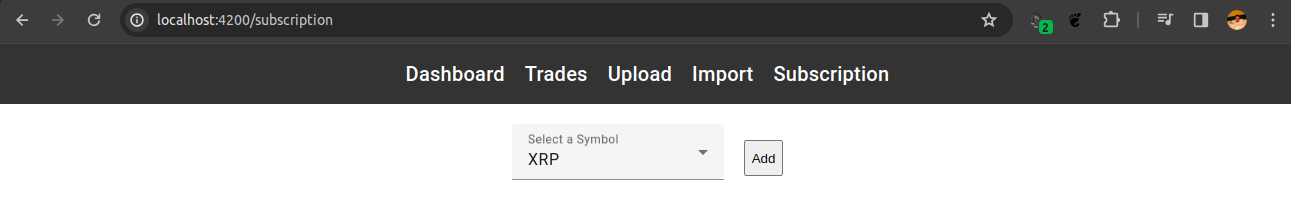
\includegraphics[width=\textwidth]{figures/frontend_subscription.png}
    \caption{Subscription}
    \label{fig:frontend_subscription}
\end{figure}

\subsubsection{Interface and Functionality}
This tab simplifies the process of adding new currency pairs for data collection:
\begin{itemize}
    \item Features a dropdown list that allows users to choose their preferred currency pair, such as \texttt{XRP}.
    \item The \texttt{Add} button is used to submit the request to the collector module, which then begins to monitor and collect data for the selected currency pair.
\end{itemize}

\subsubsection{User Empowerment}
This feature empowers users by giving them control over the scope of data collection, allowing for a personalized and relevant data set that aligns with their specific interests or trading strategies.

\subsubsection{System Scalability}
The ability to add new currency pairs on-the-fly demonstrates the system's scalability and adaptability to user needs and market changes. \\ \mbox{}
\\
In essence, the \texttt{Subscription} tab provides a vital function that ensures the system's data collection processes remain dynamic and user-driven, effectively expanding the system's analytical reach as new currency pairs are introduced into the marketplace. \\
